\documentclass[11pt, a4paper]{article}
\usepackage{graphicx} % Required for inserting images
\usepackage{caption} % for captions
\usepackage{bbm} % Math font; use \mathbbm{}
\usepackage[acronym]{glossaries} % for acronyms
\usepackage{physics} % Physics symbols

\usepackage{showlabels} % To show equations labels on the PDF. Comment at the end

% Defining acronyms
\newacronym{etk}{ETK}{Einstein Toolkit}
\newacronym{tov}{TOV}{Tolman-Oppenheimer-Volkoff}
\newacronym{ns}{NS}{neutron star}
\newacronym{iu}{IU}{internal units}
\newacronym{eos}{EOS}{equation of state}

% Defining variables
\newcommand\figifcap{Initial and final conditions}
\newcommand\figrescompcap{Resolution comparison}

\title{Numerical Relativity Homework 2}
\author{Federico Leto di Priolo}
\date{June 2024}

\begin{document}

\maketitle

\section{Sod Shock Tube Problem}

The Sod shock tube problem consists of a one-dimensional Riemann problem with initial discontinuities in density and pressure. The time evolution of the system can be computed by solving the Euler equations. Since the solution to this problem can be computed exactly, it is useful
for testing the accuracy of numerical codes. In this exercise, we solve the Sod problem with the \acrfull{etk} using different resolutions and compare the results with the exact solution.

The solution to the problem is described by three characteristics, each related to the propagation speed of the fluid in different regions. These can be associated with either a rarefaction wave, a shock wave, or a contact discontinuity. Specifically, the pressure and the velocity of the fluid develop a rarefaction wave and a shock wave, while the density also develops a contact discontinuity. The exact solution along with the initial conditions is shown in Figure \ref{fig:all_exact_if}.

For the numerical solutions, the HLLE Riemann solver has been used, along with the Minmod slope limiter. The domain extends in the range
\([-0.5, 0.5]\), and the evolution proceeds up to time \(t = 0.4\). The grid spacings used are \(\{0.005, 0.0025, 0.00125, 0.000625\}\), corresponding respectively to \(\{200, 400, 800, 1600\}\) grid points.

\subsection{Highest Resolution: 1600 points} \label{sec:highres1600}

We will use the results obtained with the highest resolution to showcase how the numerical solutions look. Figure \ref{fig:all_1600_snapshots} shows some snapshots of the profiles of density, pressure, and velocity of the fluid, including the initial and the final ones. As can be seen, S and CD waves travel in opposite directions with respect to the R waves. We point out that the fact that the initial profile in Figure \ref{fig:all_1600_snapshots} doesn't perfectly resemble a step (as it should) is due to the way the numerical results are interpolated on the chosen uniform grid \([-0.45, 0.45]\). Interpolation effects are also present in the final profile, though they are less evident. However these effects can be reduced by increasing the number of grid points of the uniform grid used for the plot. Figure \ref{fig:all_1600_initial_compare} compares the interpolated initial data with the raw initial data actually used by the \acrshort{etk}. 

The numerical solution captures the discontinuities in the physical variables observed for the Sod problem. Accuracy depends on the number of grid points, but slight smoothing of the discontinuities seems to be a characteristic feature of the HLLE Riemann solver. This also applies to the boundaries of the rarefaction wave, where the solution slope changes rapidly. This behavior isn't related to the interpolation of the data on the plot's grid, as shown in the next section (\ref{sec:rescomp}).

\subsection{Resolutions Comparison} \label{sec:rescomp}

Now we examine the results obtained with different resolutions and compare them to the exact solution. To avoid visualization artifacts, we will use the raw data from the \acrshort{etk} and not the interpolated ones. Figures \ref{fig:rho_final_rescompare}, \ref{fig:press_final_rescompare}, and \ref{fig:vel_final_rescompare} show the final iteration of the evolution of density, pressure, and velocity respectively.

As mentioned in the previous section (\ref{sec:highres1600}), the smoothing of the discontinuities appears to be a feature of the Riemann solver rather than of the chosen resolution. At the same time, as expected, it is indeed true that a finer spacing of the numerical grid reduces the observed smoothing. Moreover, we point out that there are no evident numerical oscillations near the discontinuities for any of the resolutions used.

Overall, considering its simplicity and low computational cost, the HLLE solver showed good handling of the Sod problem resolution. However, simulations where a higher shock resolution is needed, might require more advanced Riemann solvers.

\newpage

\begin{center}
    \centering
    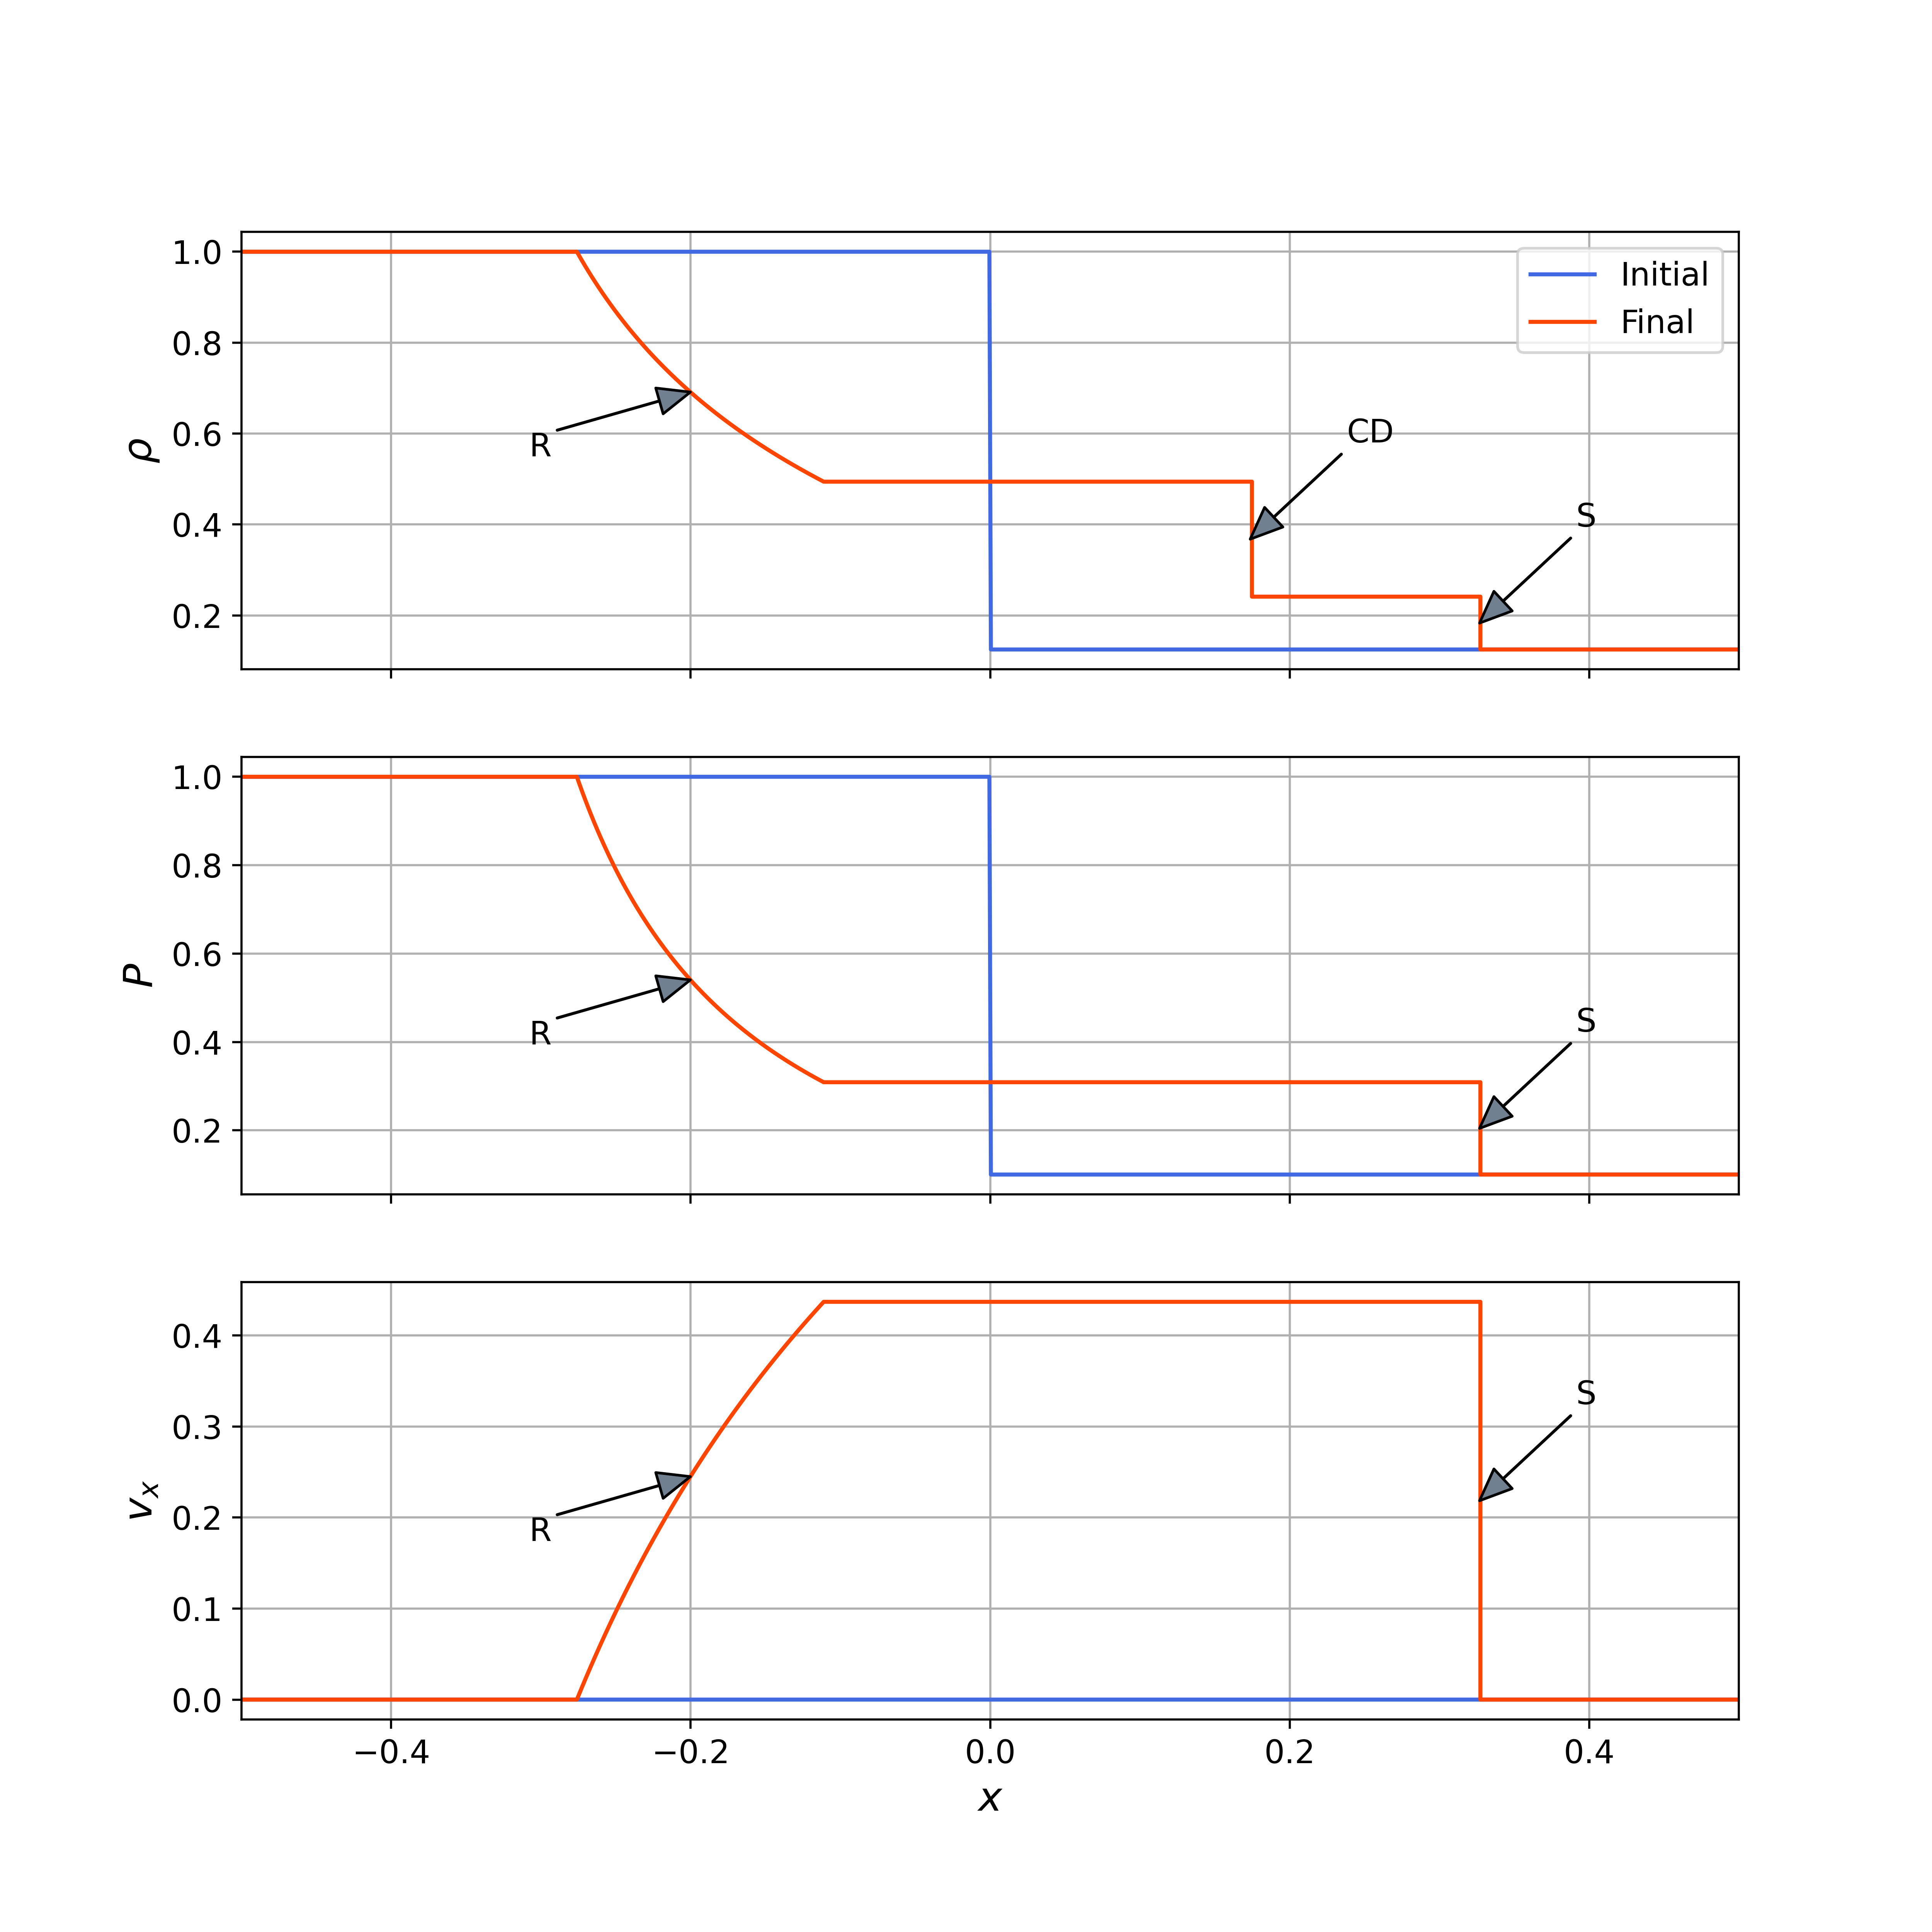
\includegraphics[width=1\linewidth]{images/all_exact_if.png}
    \captionof{figure}{Exact Solution; \figifcap; The arrows points at the different types of waves: R (Rarefaction), S (Shock) and CD (Contact Discontinuity).}
    \label{fig:all_exact_if}
\end{center}

\begin{center}
    \centering
    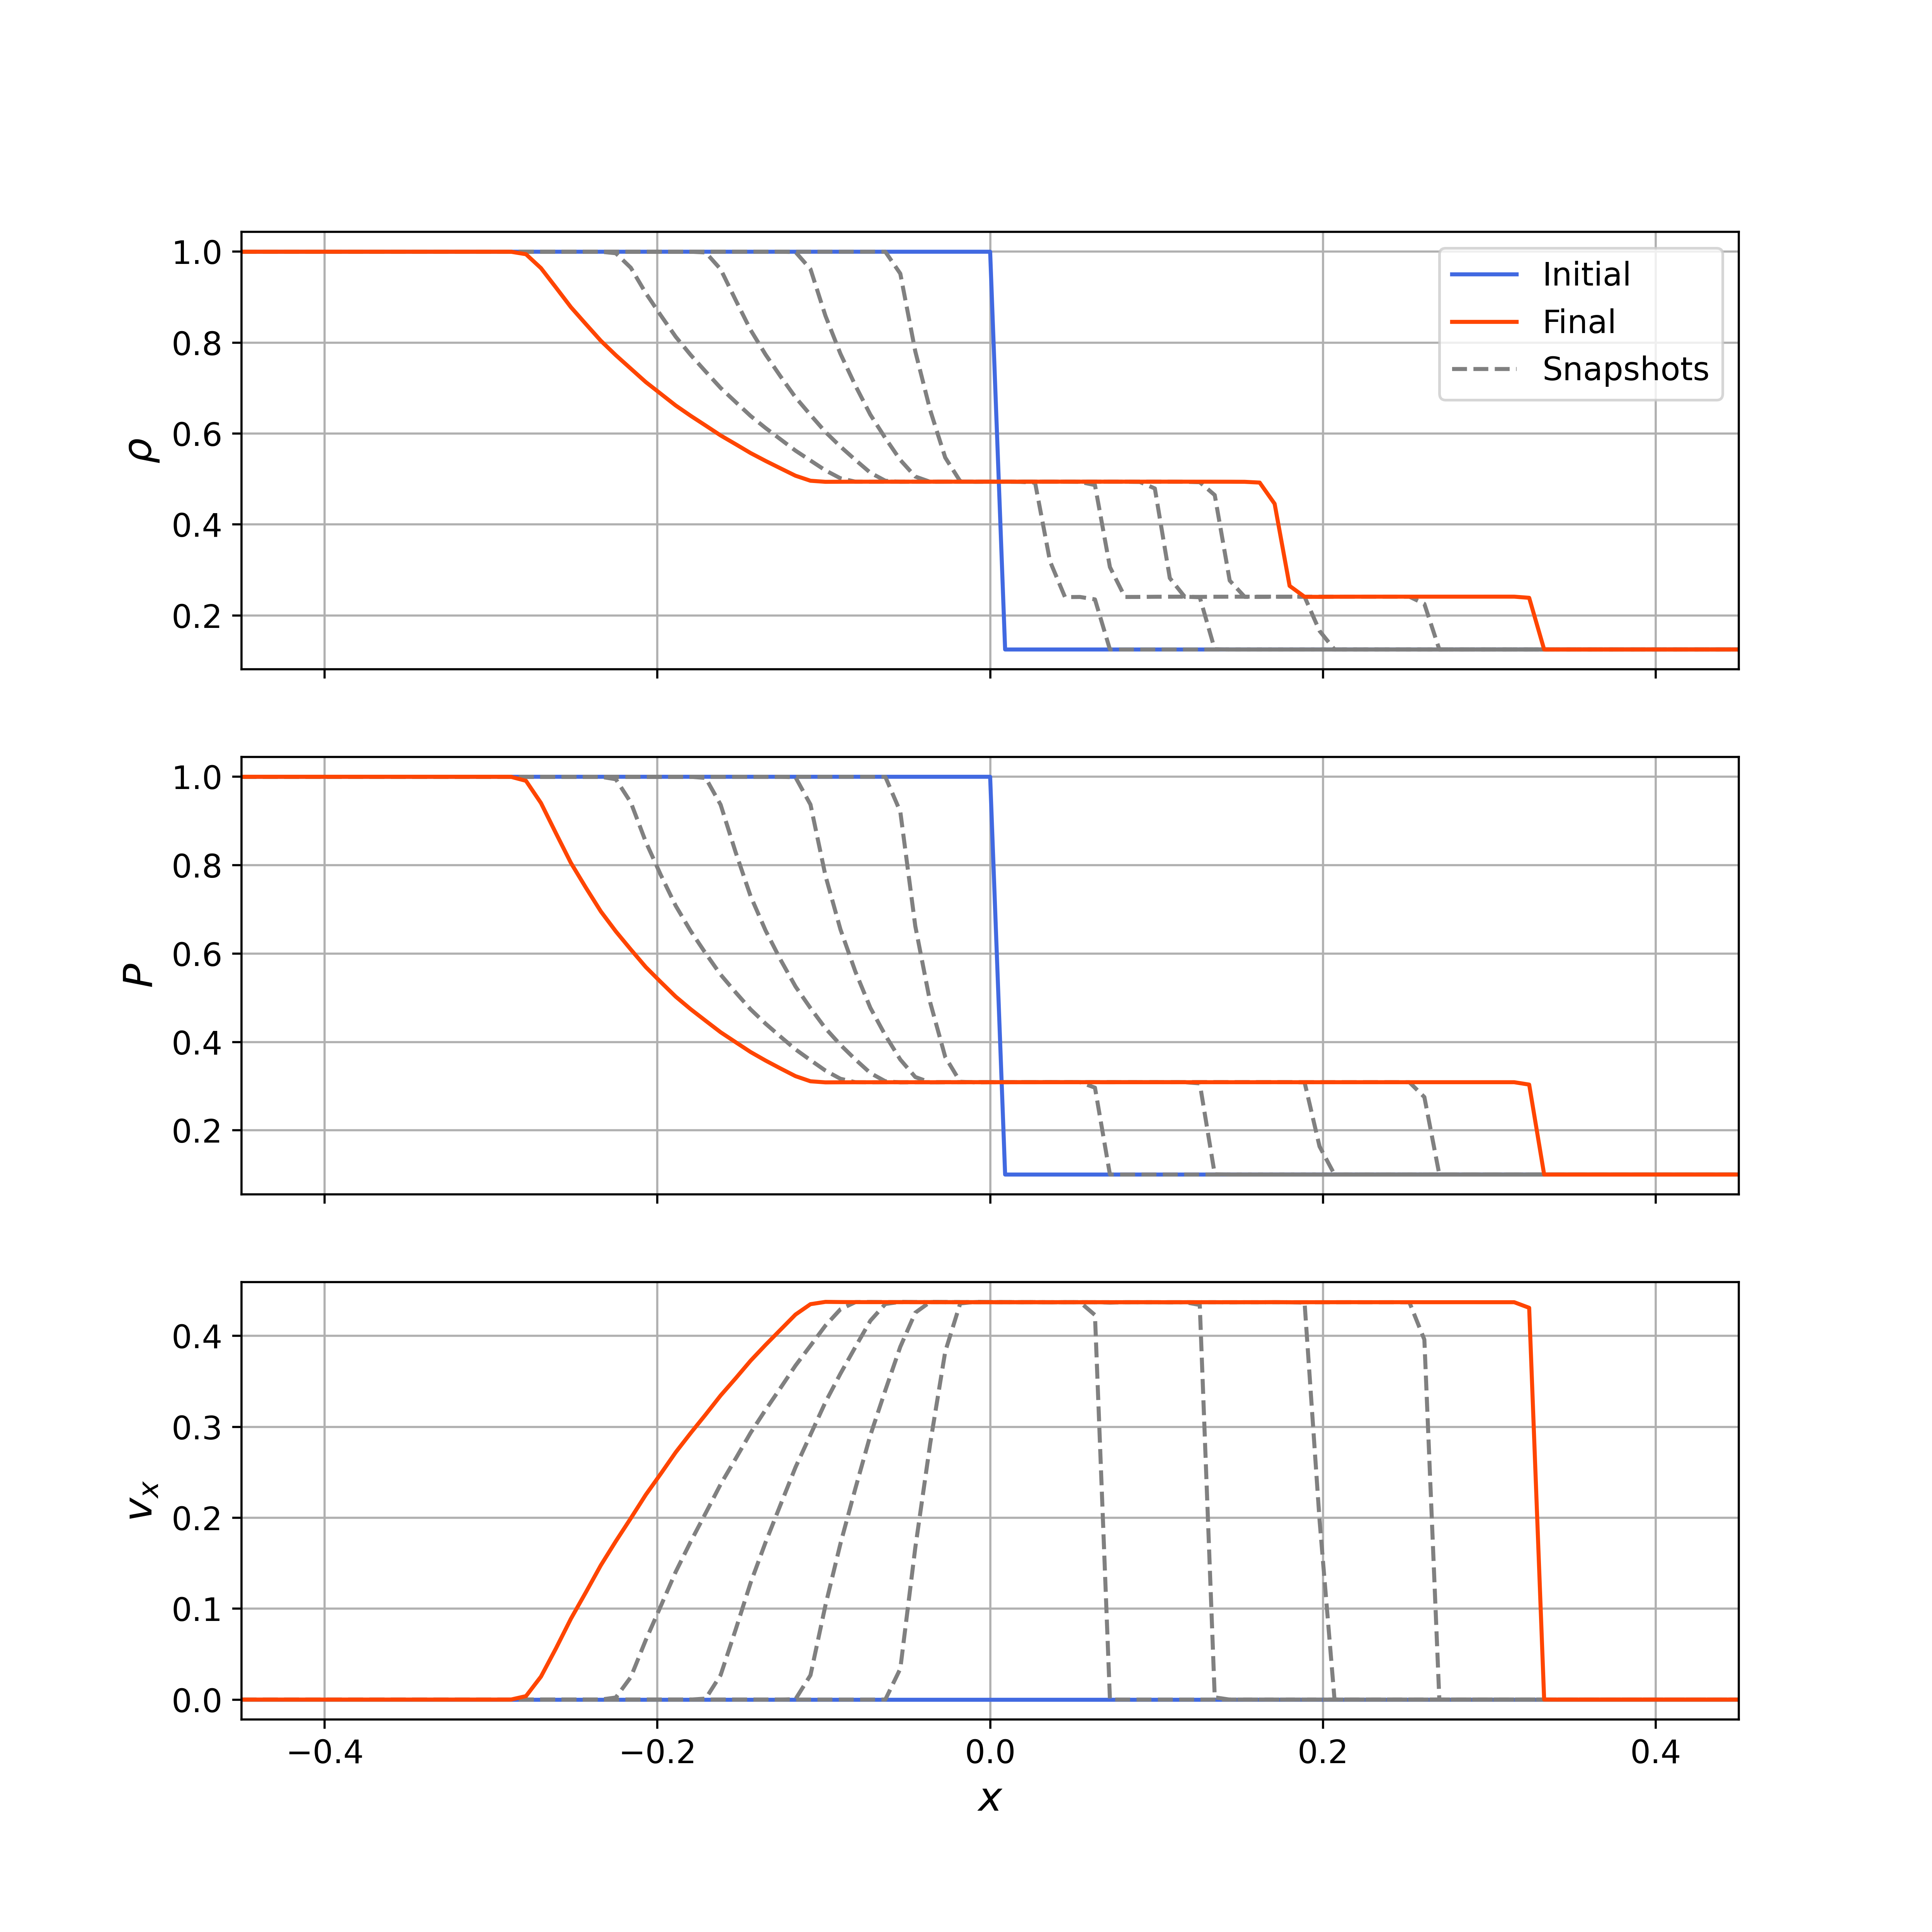
\includegraphics[width=1\linewidth]{images/all_1600_snapshots.png}
    \captionof{figure}{Numerical Solution; 1600 points; Snapshots.}
    \label{fig:all_1600_snapshots}
\end{center}

\begin{center}
    \centering
    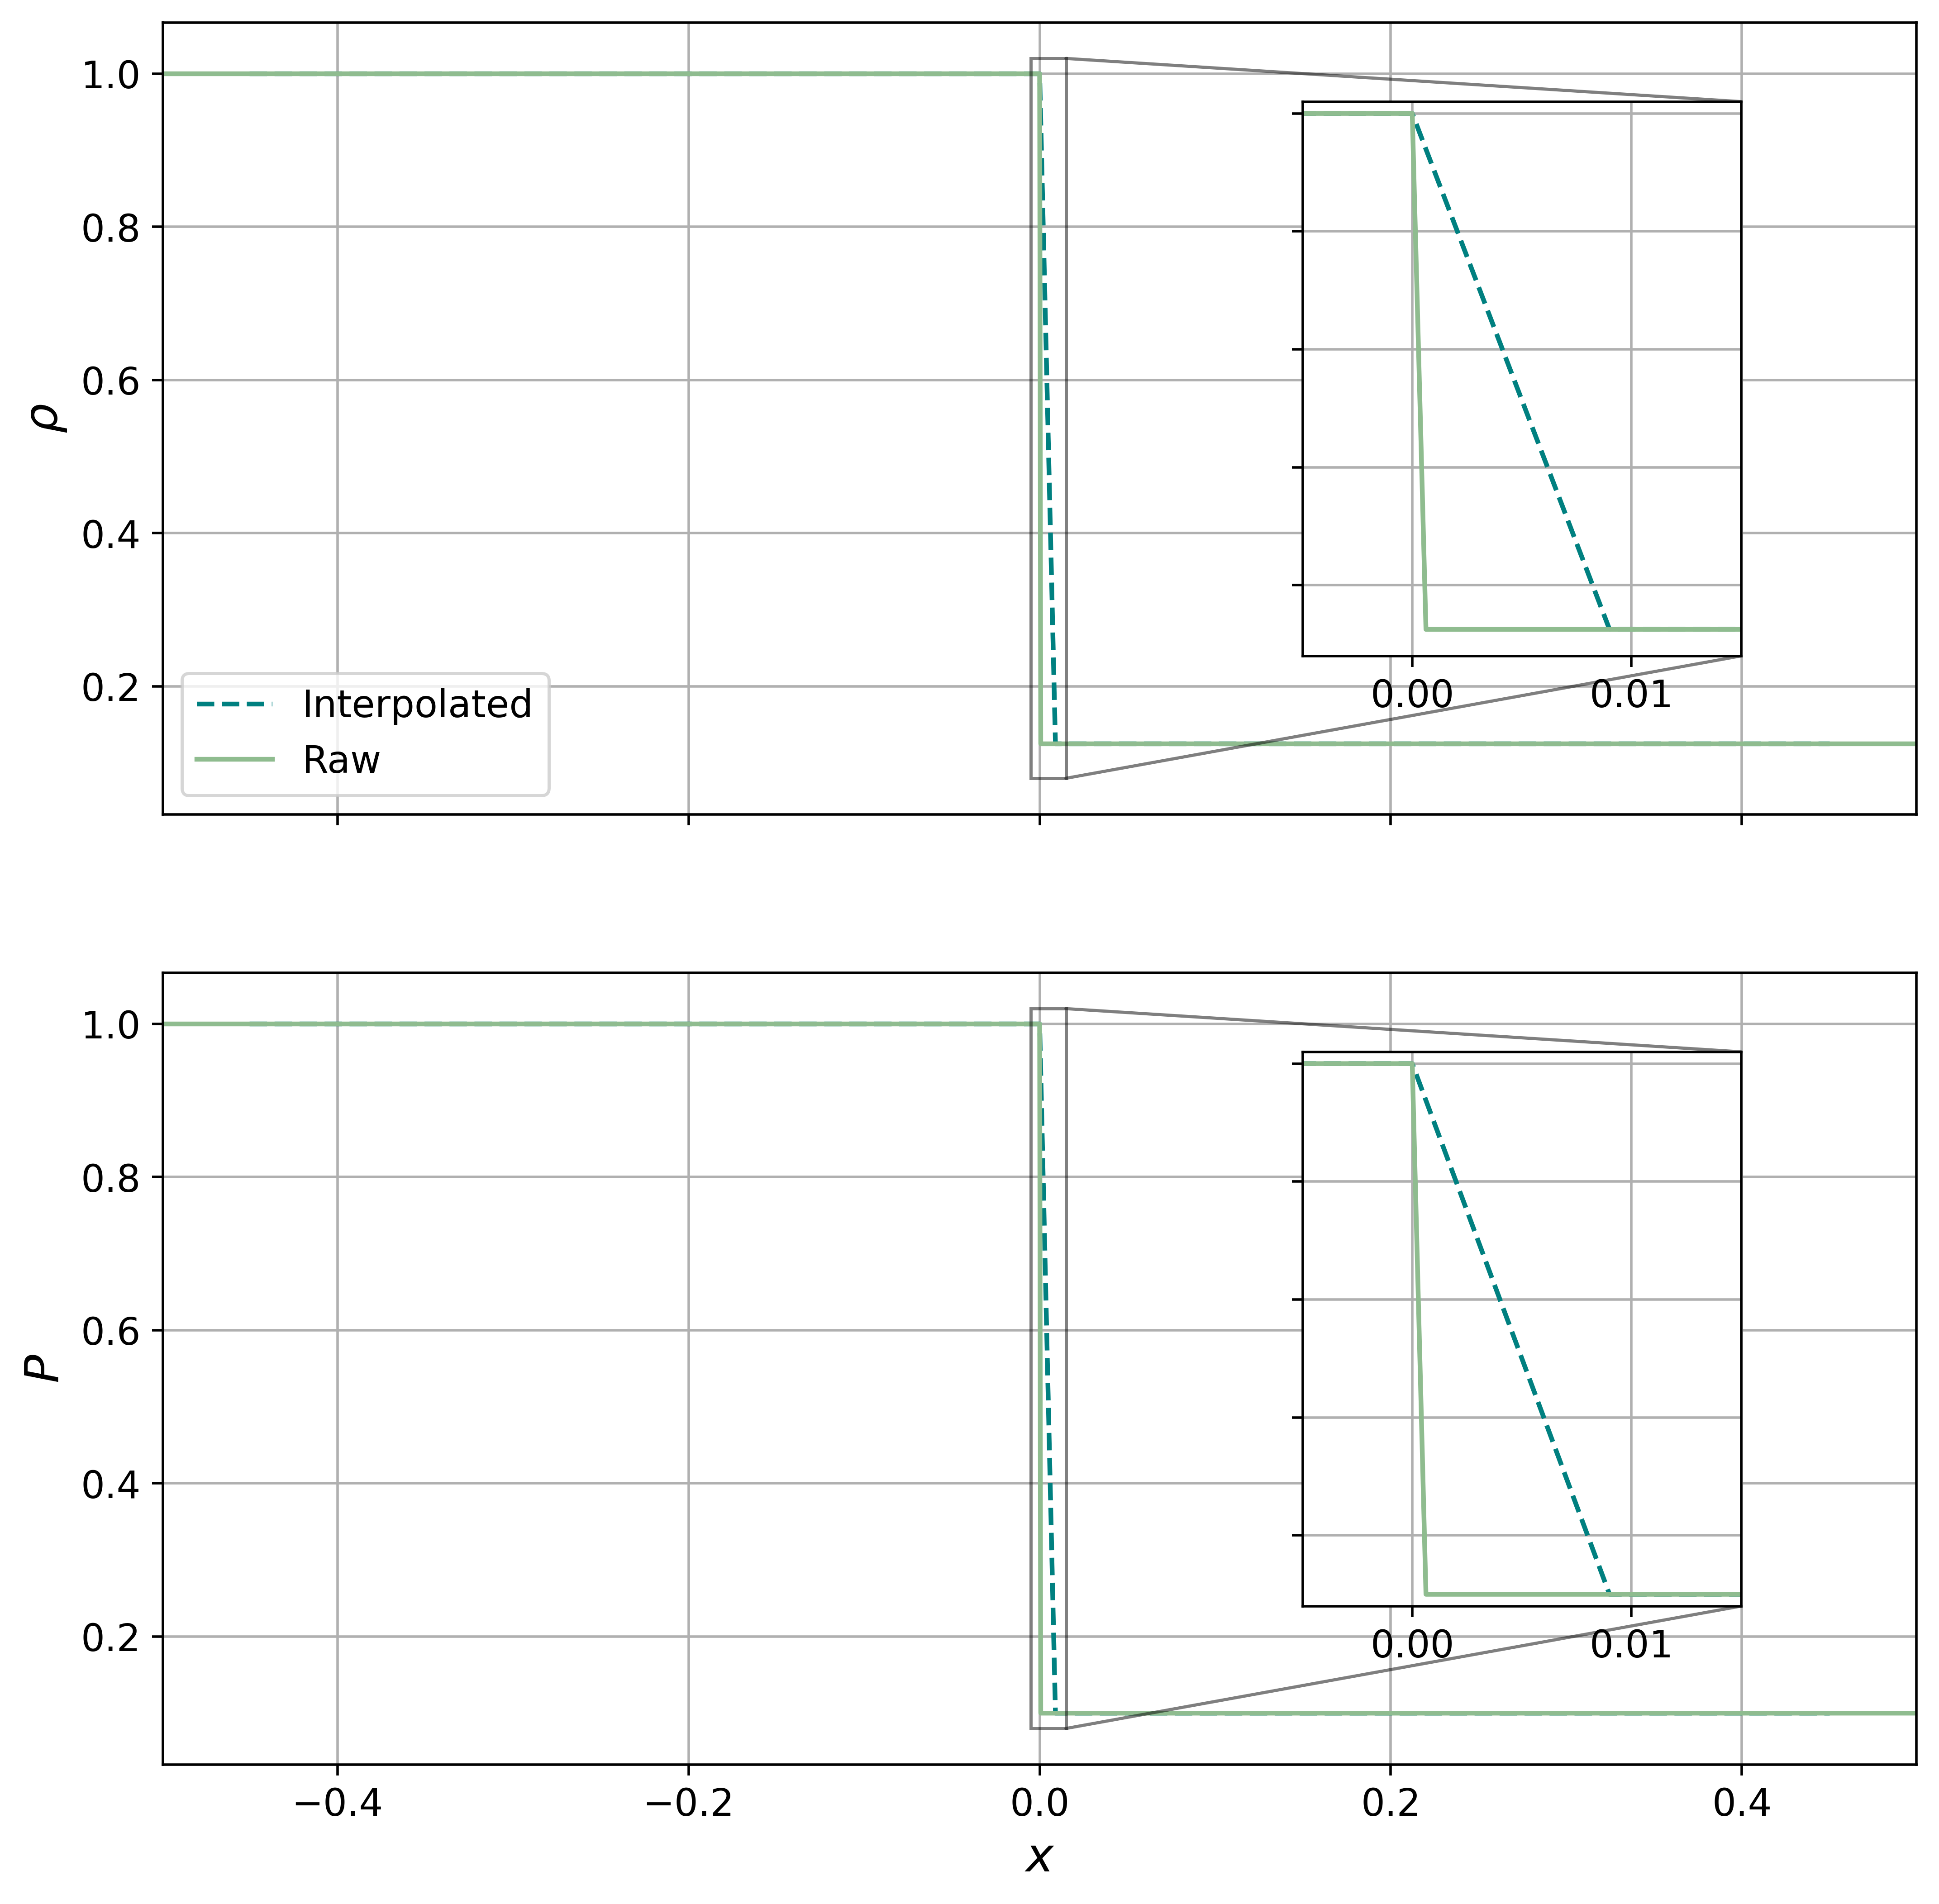
\includegraphics[width=1\linewidth]{images/all_1600_initial_compare.png}
    \captionof{figure}{Initial data; 1600 points; Raw and interpolated.}
    \label{fig:all_1600_initial_compare}
\end{center}

\begin{center}
    \centering
    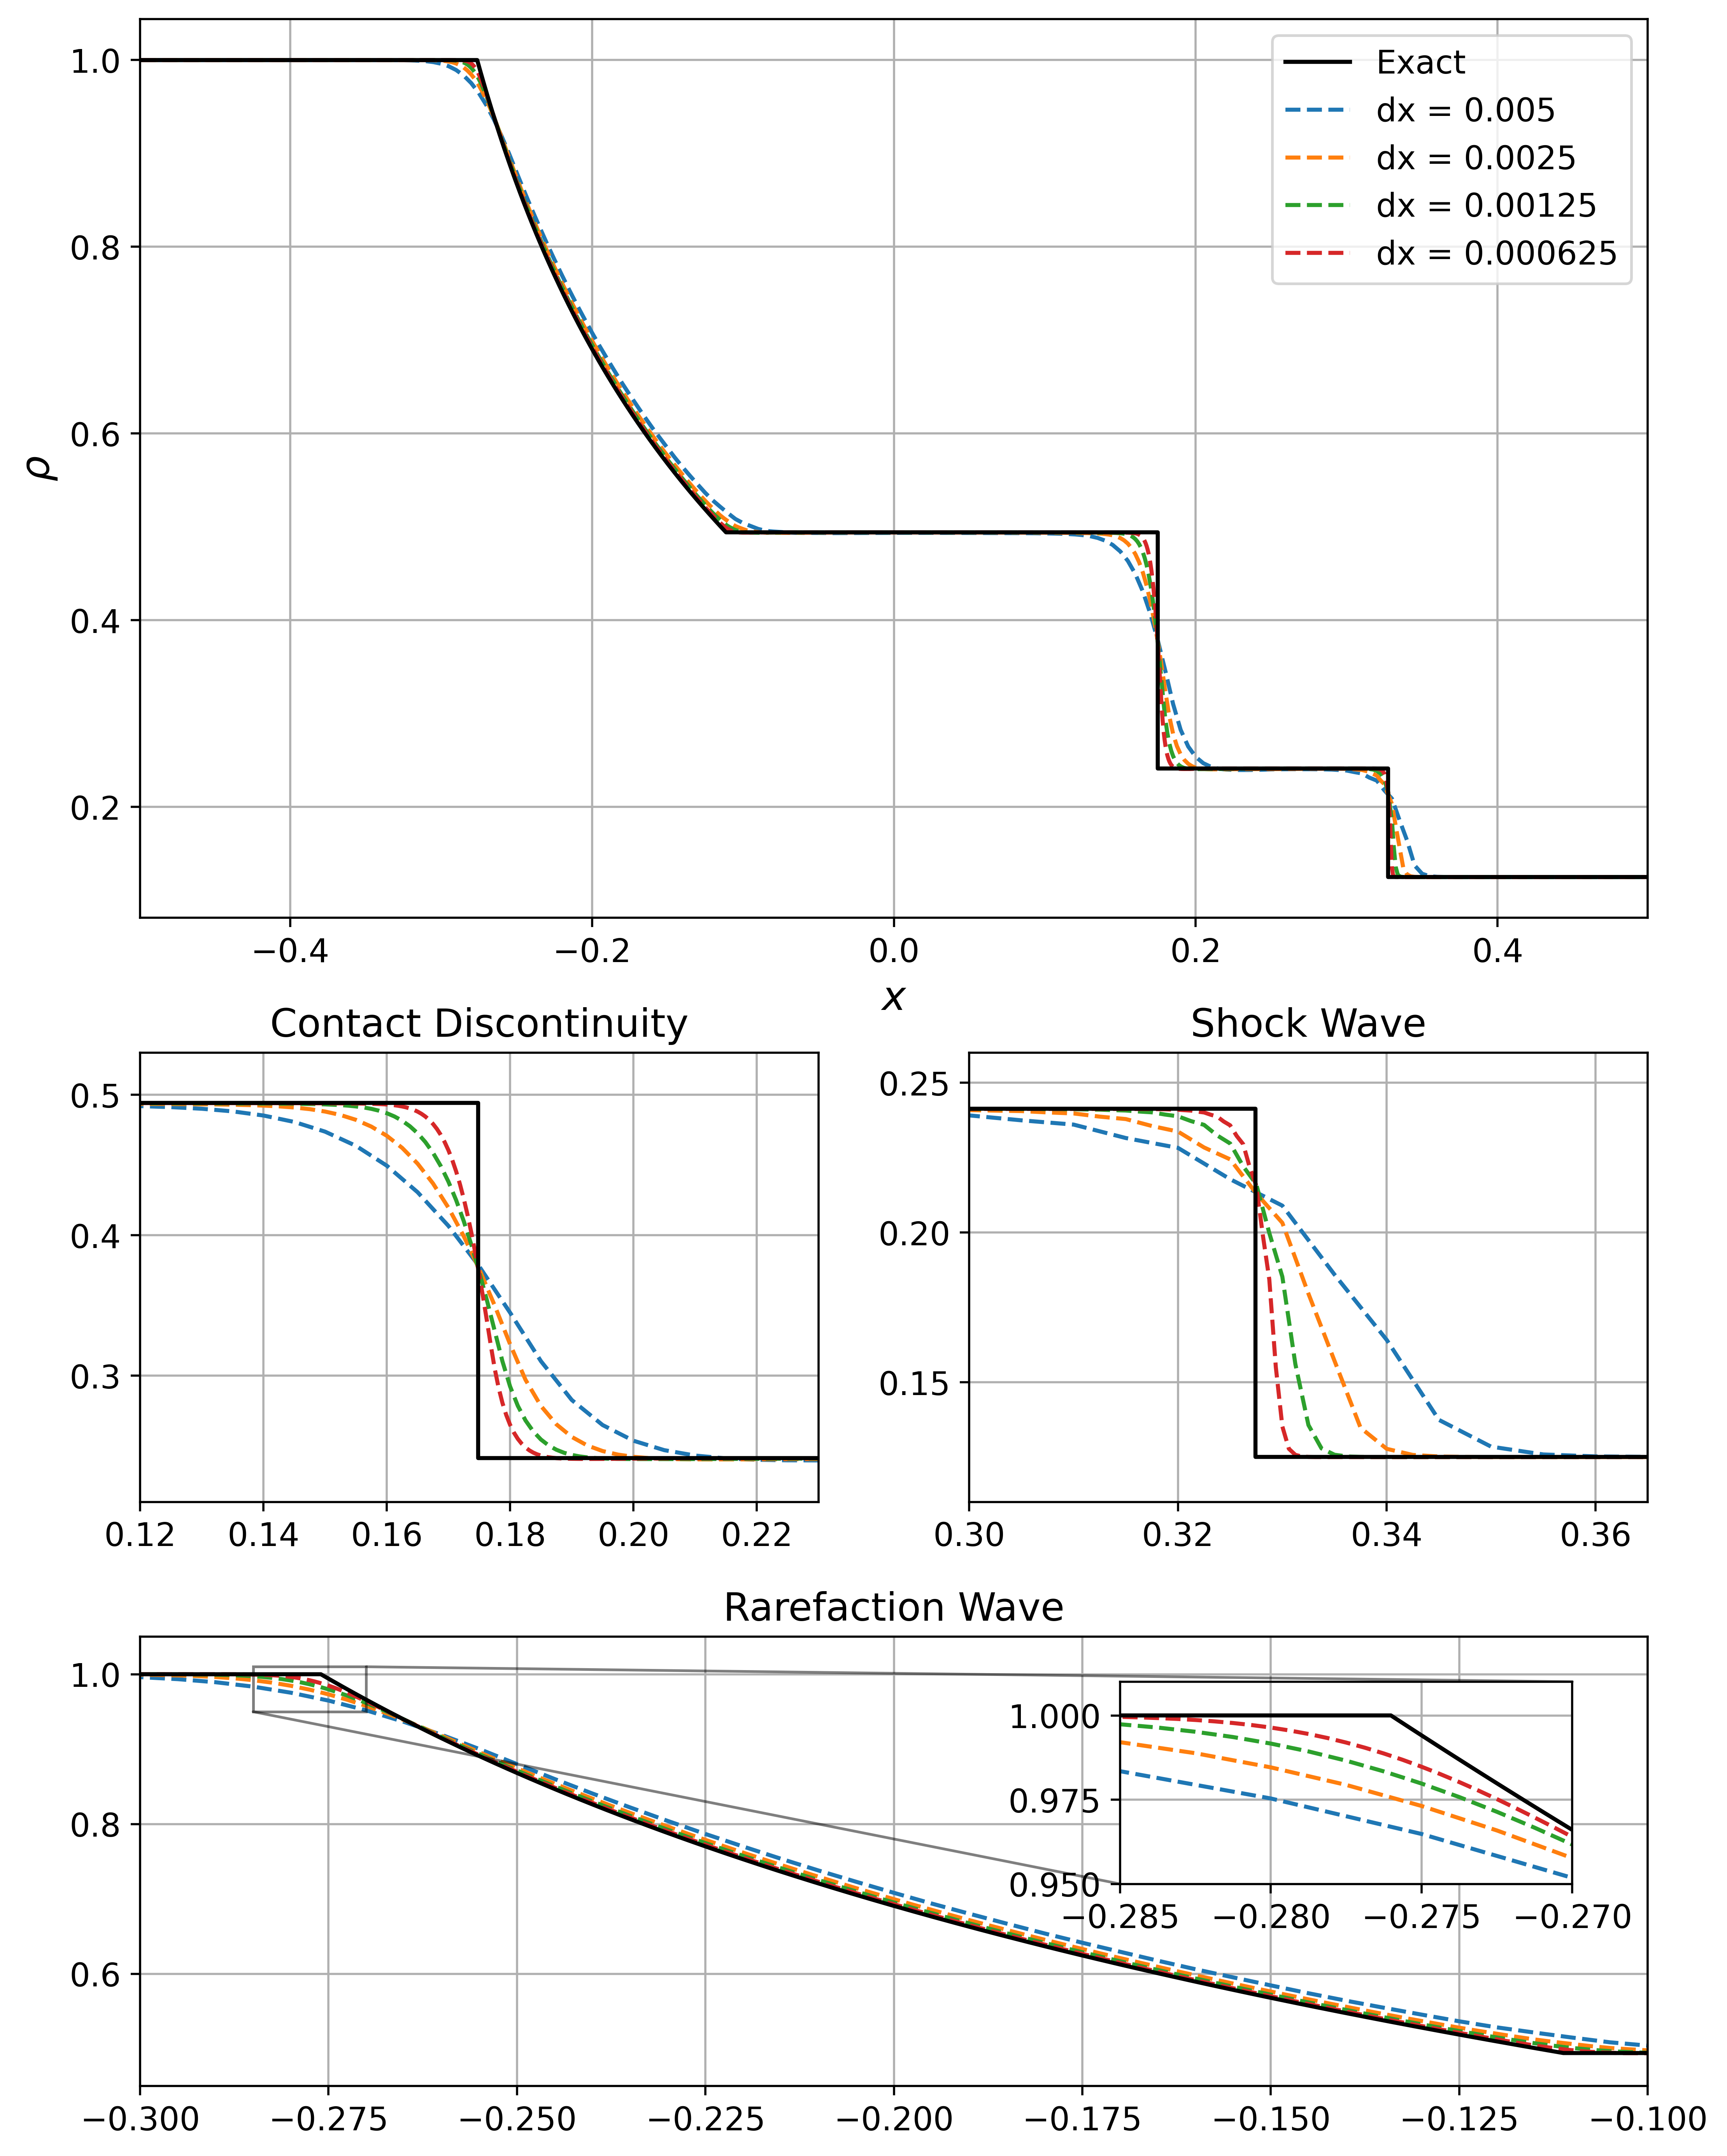
\includegraphics[width=1\linewidth]{images/rho_final_rescompare_raw.png}
    \captionof{figure}{Density; Final data; \figrescompcap.}
    \label{fig:rho_final_rescompare}
\end{center}

\begin{center}
    \centering
    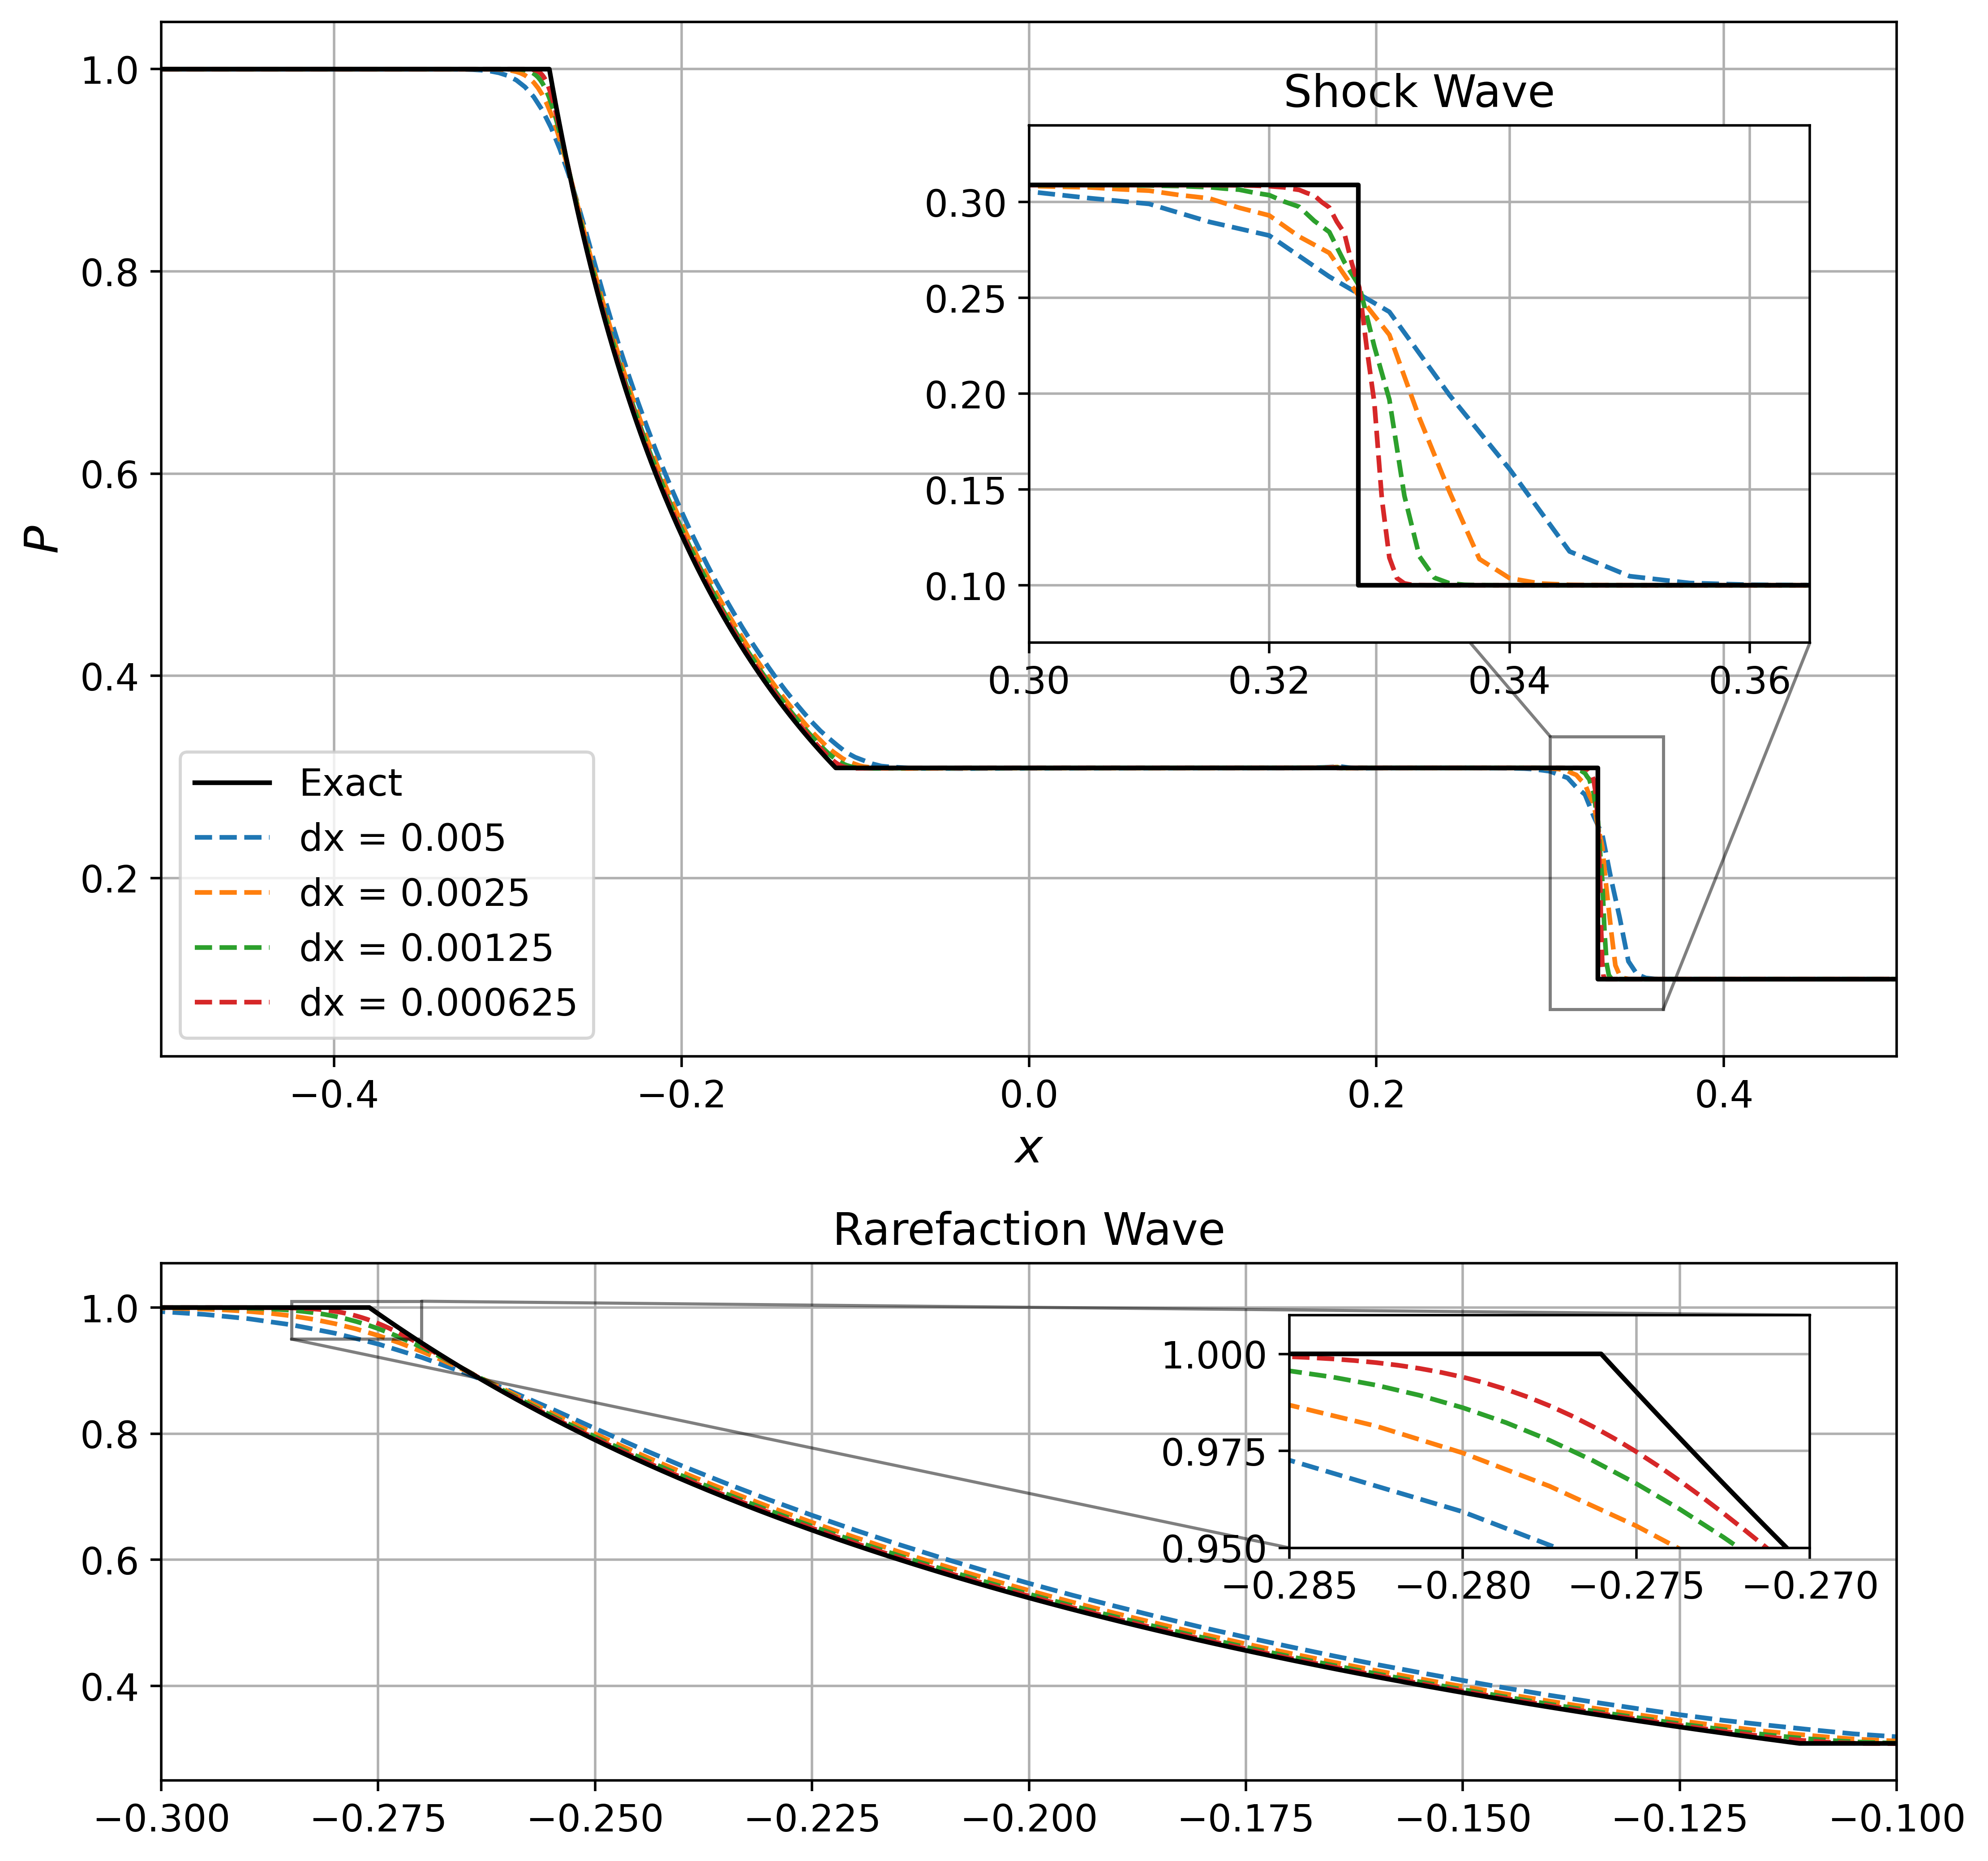
\includegraphics[width=1\linewidth]{images/press_final_rescompare_raw.png}
    \captionof{figure}{Pressure; Final data; \figrescompcap.}
    \label{fig:press_final_rescompare}
\end{center}

\begin{center}
    \centering
    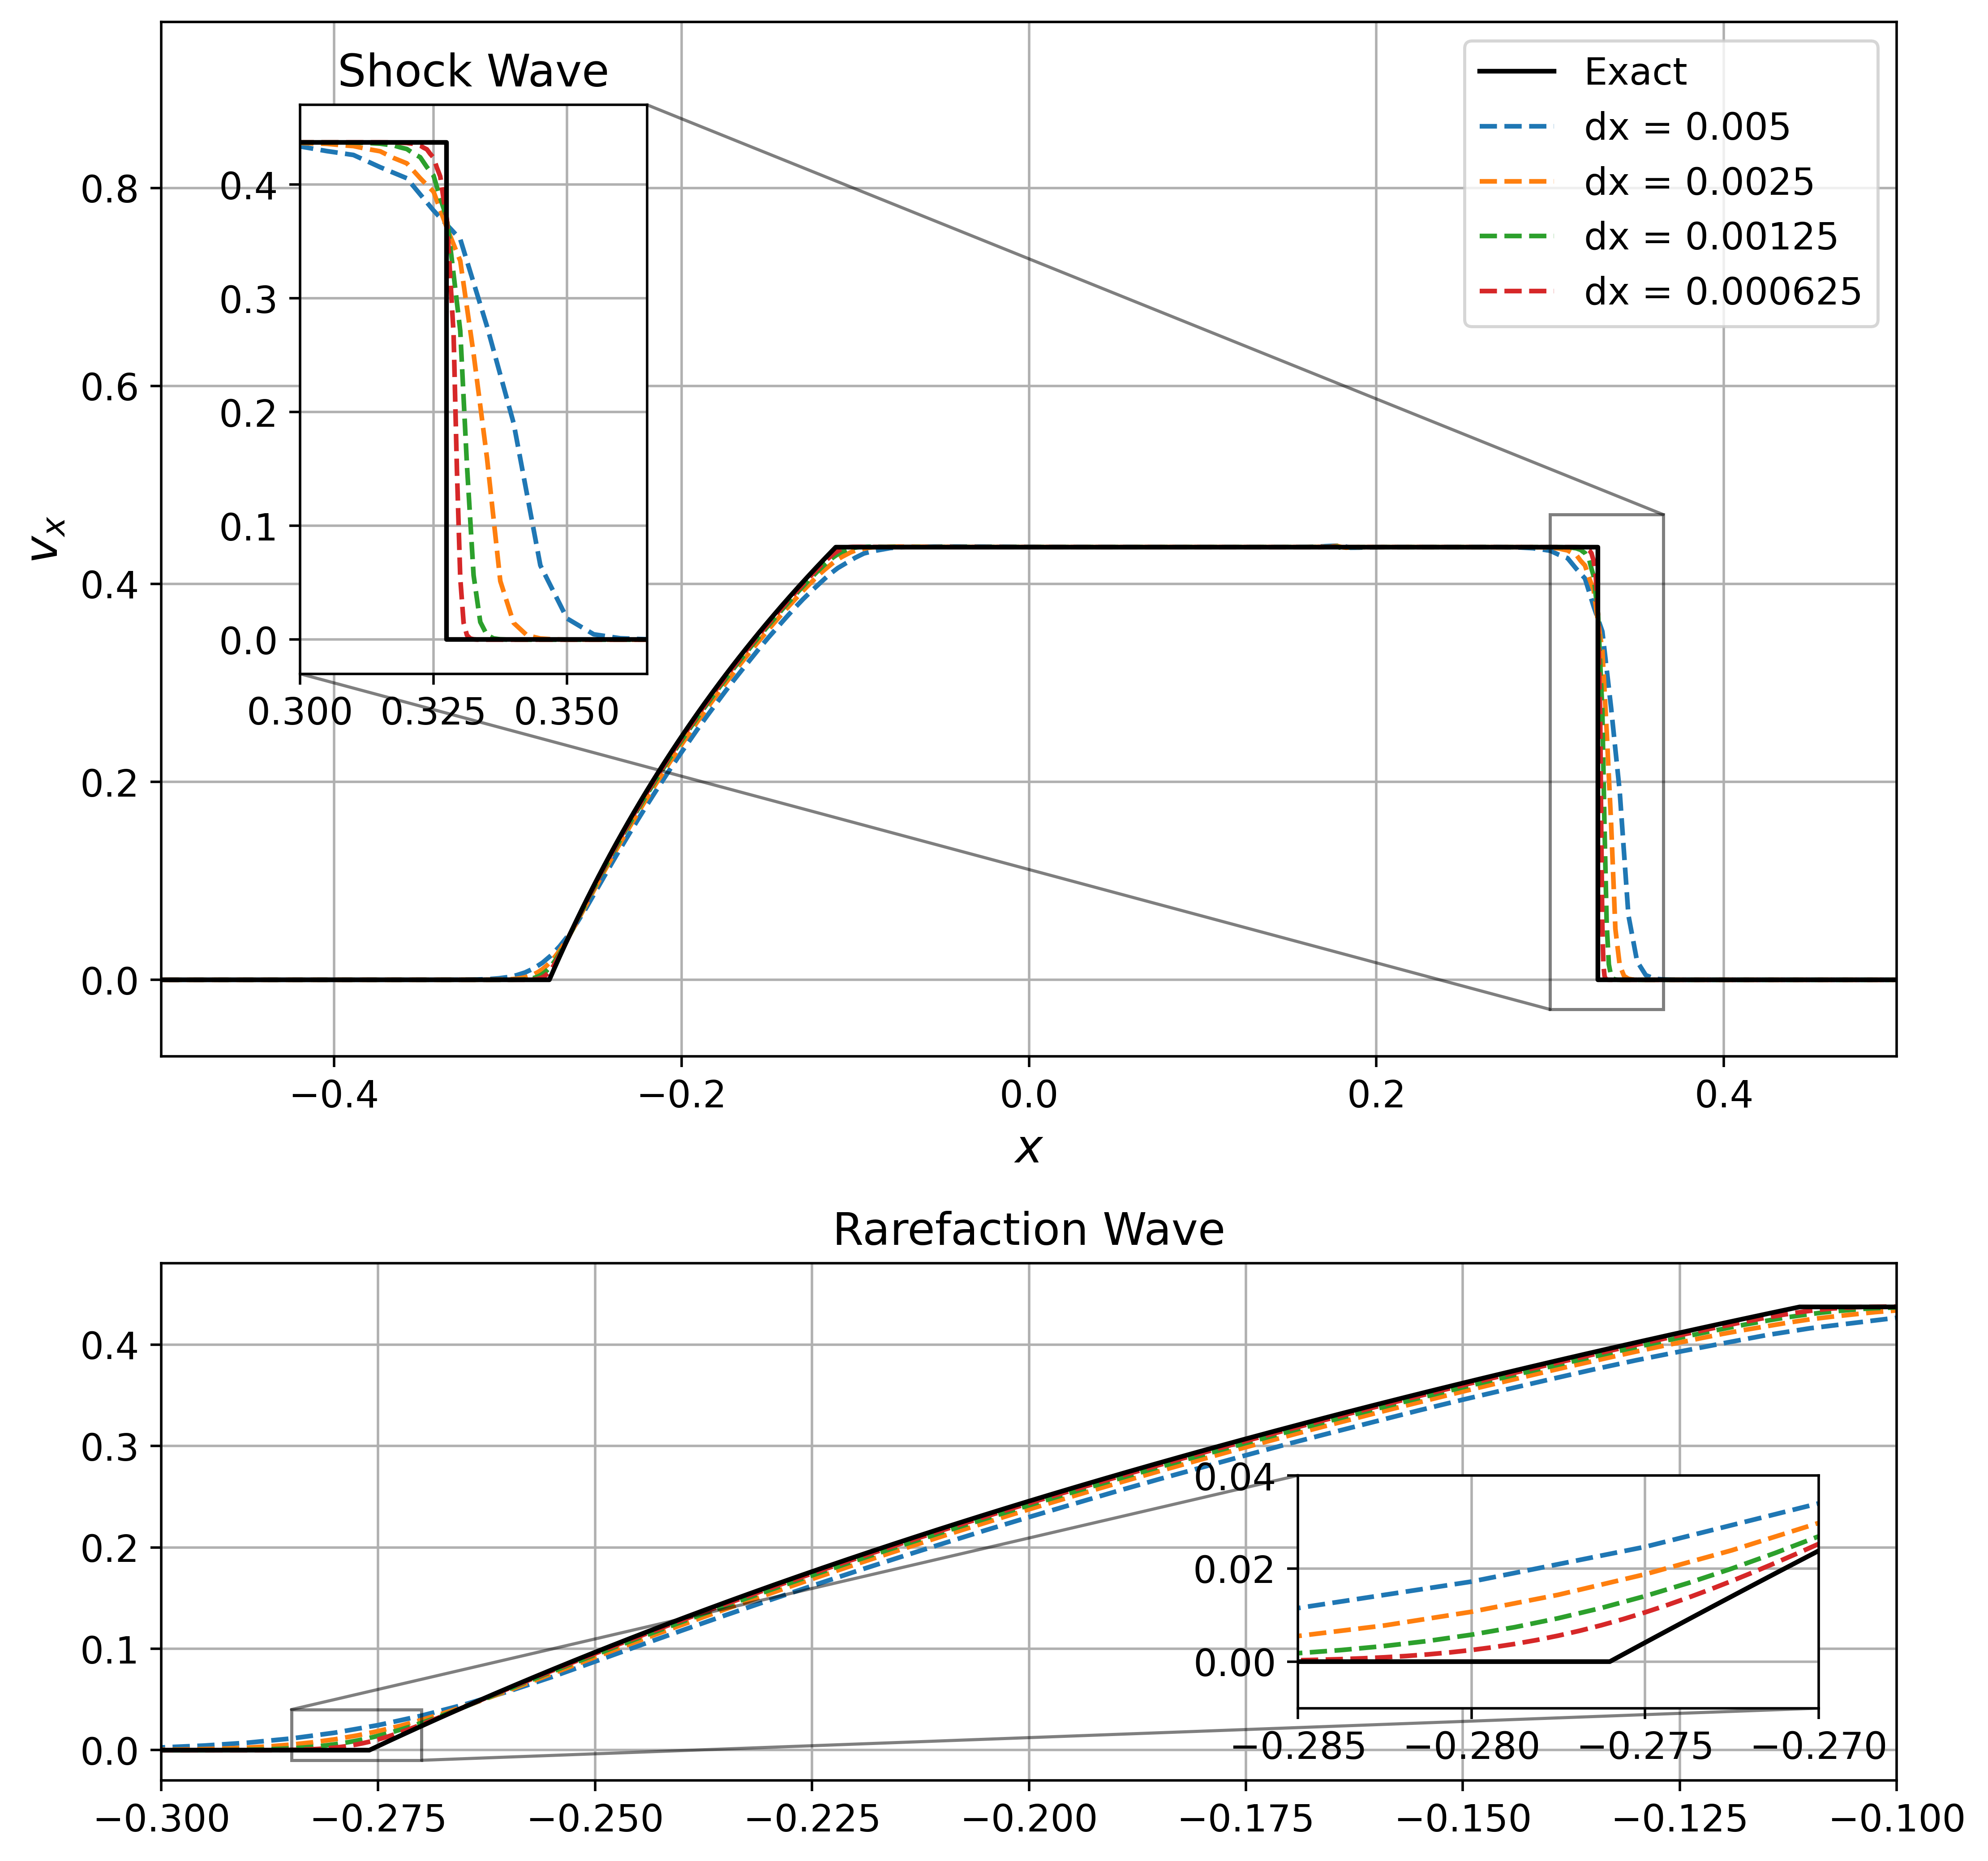
\includegraphics[width=1\linewidth]{images/vel[0]_final_rescompare_raw.png}
    \captionof{figure}{Velocity; Final data; \figrescompcap.}
    \label{fig:vel_final_rescompare}
\end{center}

\newpage

\section{TOV Evolution}

The \acrfull{tov} equation describes the physical properties of a spherically symmetric body in hydrostatic equilibrium under its own gravity. In this exercise, we study the evolution of the central value of the rest mass density (\(\rho_c\)) of a stable \acrfull{ns} using the \acrshort{etk}. The exercise is divided into two parts: in the first part, we evolve the system using different resolutions to study the numerical effects on the simulations; in the second part, we also introduce a pressure perturbation and analyze the response of the star.

The input and output of the thorns used for the evolution are in geometric units: \(G = c = M_\odot = 1\). We provide some conversion factors to convert from \acrfull{iu} to physical units for the variables we are interested in:

\begin{itemize}
    \item \textit{Length} from [\(\mathrm{M_\odot}\)] to \([\mathrm{km}]\): multiply by \(1.477\)
    \item \textit{Time} from [\(\mathrm{M_\odot}\)] to \([\mathrm{ms}]\): multiply by \(4.926 \times 10^{-3}\)
    \item \textit{Density} from [\(\mathrm{M_\odot^{-2}}\)] to \([\mathrm{g\ cm^{-3}}]\): multiply by \(6.176 \times 10^{17}\)
\end{itemize}

\noindent
In every part of the exercise, the final time of the simulation is set to \(400\ \mathrm{M_\odot}\) or about \(2\ \mathrm{ms}\). The \acrshort{ns} is centered at the origin of the reference frame, and the numerical grid spans in each direction the \([0, 24]\ \mathrm{M_\odot}\) interval, which corresponds roughly to a \(35\ \mathrm{km}\) side cube. The evolution of the equations in the regions of the stars outside of the grid domain is handled by the \textit{ReflectionSymmetry} thorn which mirrors the solution computed in the 3-dimensional \([0, 24]\) cube using the spherical symmetry of the problem. In every simulation, there is also one refinement level set on the \([0, 12]\ \mathrm{M_\odot}\) interval, having twice the starting resolution. For both parts of the exercise, a simulation has been run with each of the following grid spacing of the main grid in each of the three Cartesian directions: \(\{2.0, 1.0, 0.5\}\).

\subsection{Changing the resolution}

Figure \ref{fig:ns_rho_init_rescompare} shows the projection on the \(xy\) plane of the rest mass density of the initialized \acrshort{ns} with each of the used resolutions. The spherical symmetry of the problem is clearly broken by the discrete numerical grid we are using in the simulation. However, the higher the resolution, the better the star resembles a perfect sphere on the grid. This has direct effects on the numerical evolution of the \acrshort{ns}. Outside of the \acrshort{ns}, the value of the density is constant around \(10^{8}\ \mathrm{g\ cm^{-3}}\). This is because its minimum value has been manually set to \(10^{-10}\ \mathrm{M_\odot^{-2}}\) in the parameter file.

Figure \ref{fig:ns_rhoc_0_rescompare} shows the evolution in time of the central value of the density with the used resolutions. Since no physical dissipation effect is taken into account in the simulation, if the spherical symmetry of the problem were preserved, then we'd expect the central density to stay constant in time. However, the fact that the star is discretized on the grid leads to the oscillations we observe. The lower the resolution, the further the star is from spherical symmetry, the greater the oscillations it experiences to adapt to the discretized space it lies in.

\subsection{Pressure perturbation}

In the second part of the exercise, we introduced a pressure perturbation in the evolving \acrshort{ns} by modifying the \textit{poly\_k} parameter of the \textit{EOS\_Omni} thorn. This means modifying the \(K\) coefficient in the polytropic \acrfull{eos} (Equation \ref{eq:poly_eos}) used to evolve the \acrshort{tov} solution:

\begin{equation} \label{eq:poly_eos}
    p = K \rho^\gamma
\end{equation}

\noindent
where \(K\) is the polytropic constant, and \(\gamma\) is the adiabatic index. The \acrlong{ns} has been initialized using \(K = 100\), while the \acrshort{eos} for the evolution has \(K = 110\). The simulations have been run using the same resolutions as before and the initial conditions are also unchanged (same as Figure \ref{fig:ns_rho_init_rescompare}).

Figure \ref{fig:ns_rhoc_pert_110_rescompare} shows the time evolution of the central density for the used grid spacings. The introduction of a pressure perturbation modifies the hydrostatic equilibrium of the \acrshort{ns}; the star tries to regain equilibrium, resulting in radial pulsations proportional to the amplitude of the perturbation. Figure \ref{fig:ns_radial_pulsations} shows some snapshots of the matter distribution of the \acrshort{ns} during the simulation for the finest spacing used. As already mentioned, since the star matter is treated as a perfect fluid and the simulation doesn't take into account any dissipation effects, the amplitude of the oscillations should stay constant in time. This is not the case because of the discreteness of the numerical simulation. In fact, we notice some evident damping for the low resolution case, while it is much weaker when the resolution gets increased.
However, we point out that pure numerical oscillations in the perturbed case are a minor effect with respect to the physical ones. Figure \ref{fig:ns_rhoc_all_compare} shows the central density evolution for the perturbed and the unperturbed cases plotted together in terms of relative percentage variation from the initial value.

\newpage

\begin{center}
    \centering
    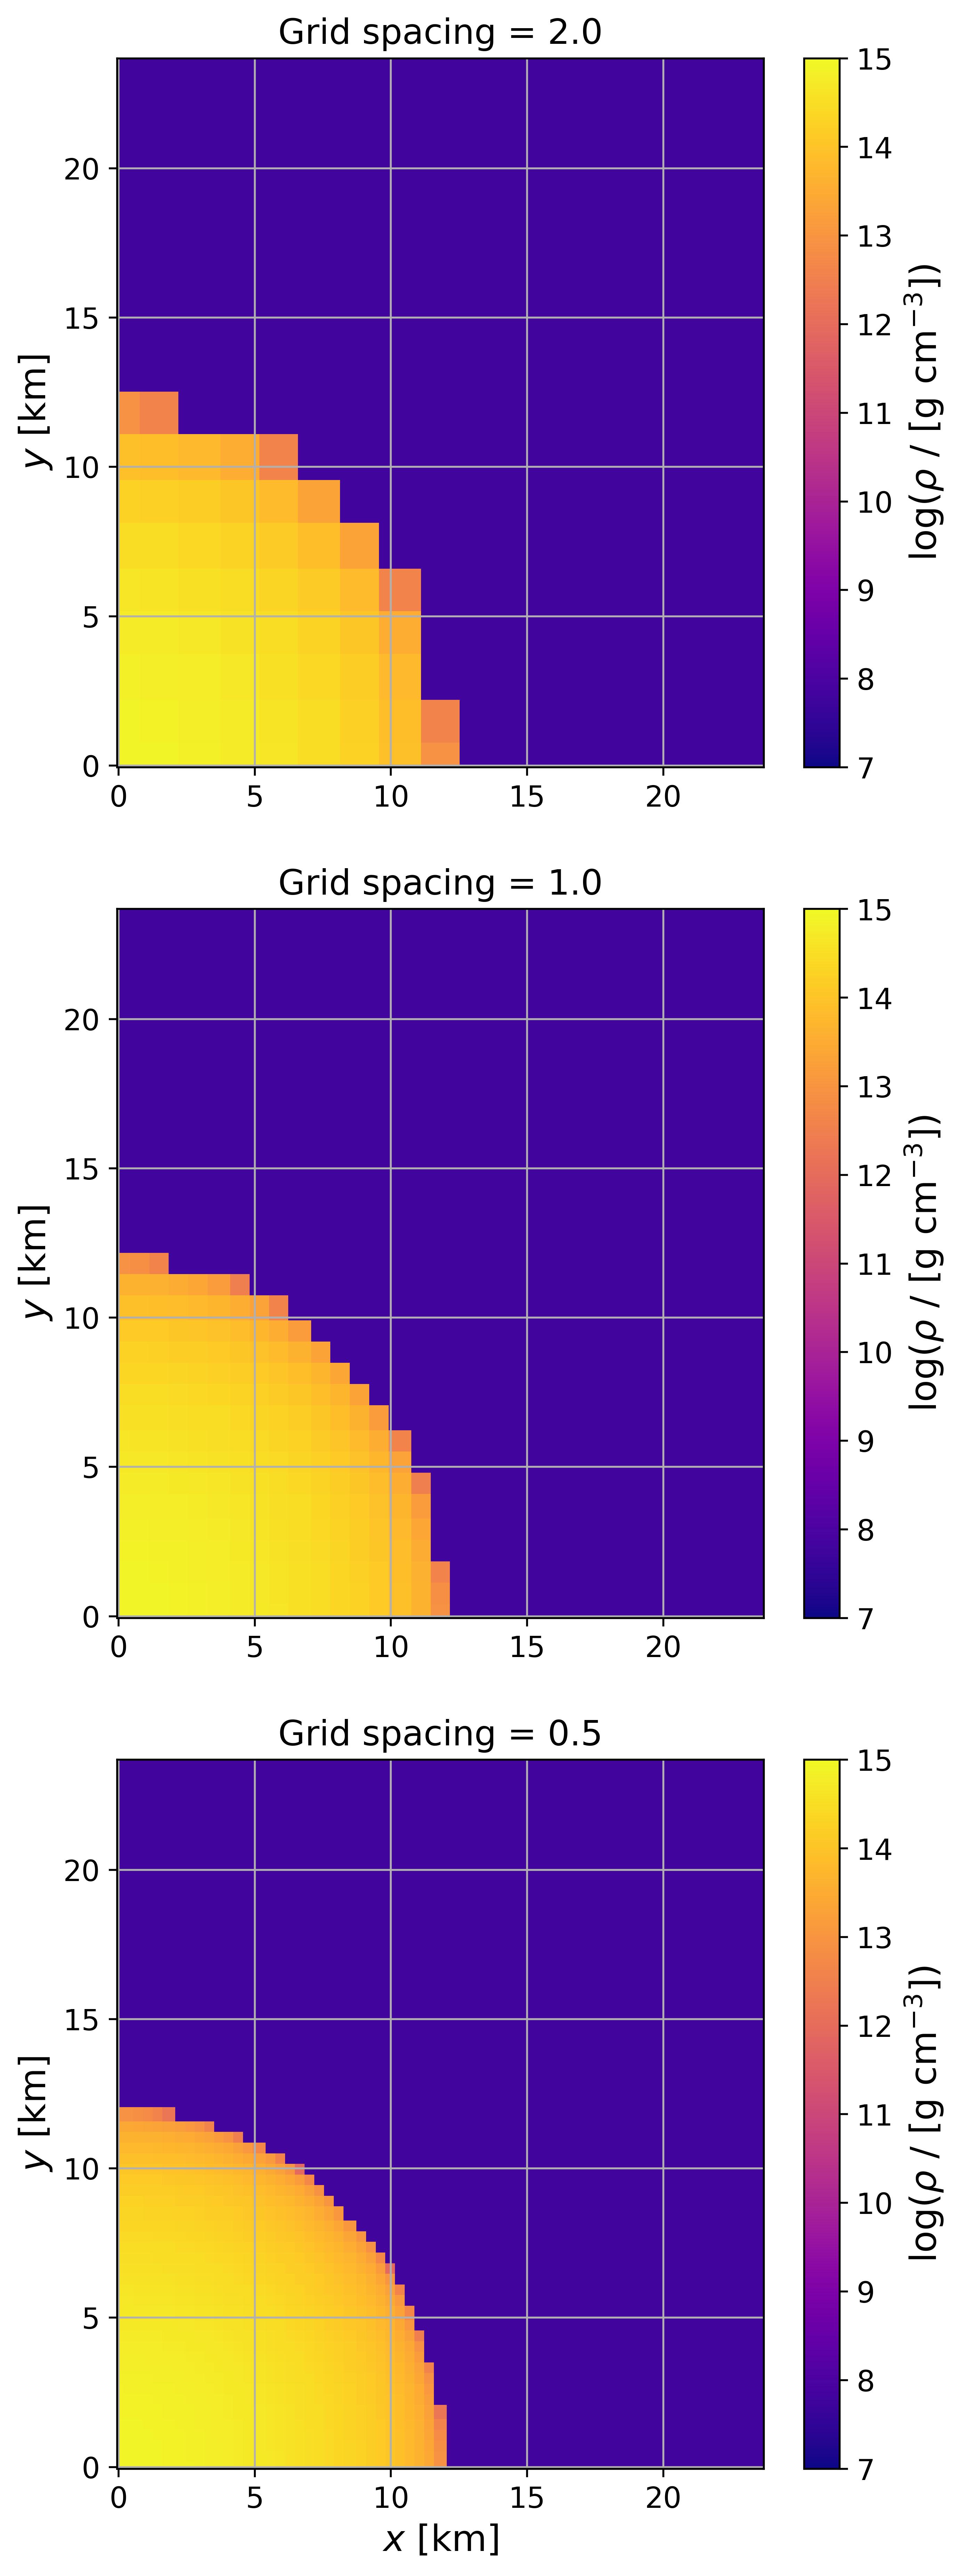
\includegraphics[height=0.9\textheight]{images/rho_init_rescompare.png}
    \captionof{figure}{Rest mass density; Initial data; \figrescompcap.}
    \label{fig:ns_rho_init_rescompare}
\end{center}

\begin{center}
    \centering
    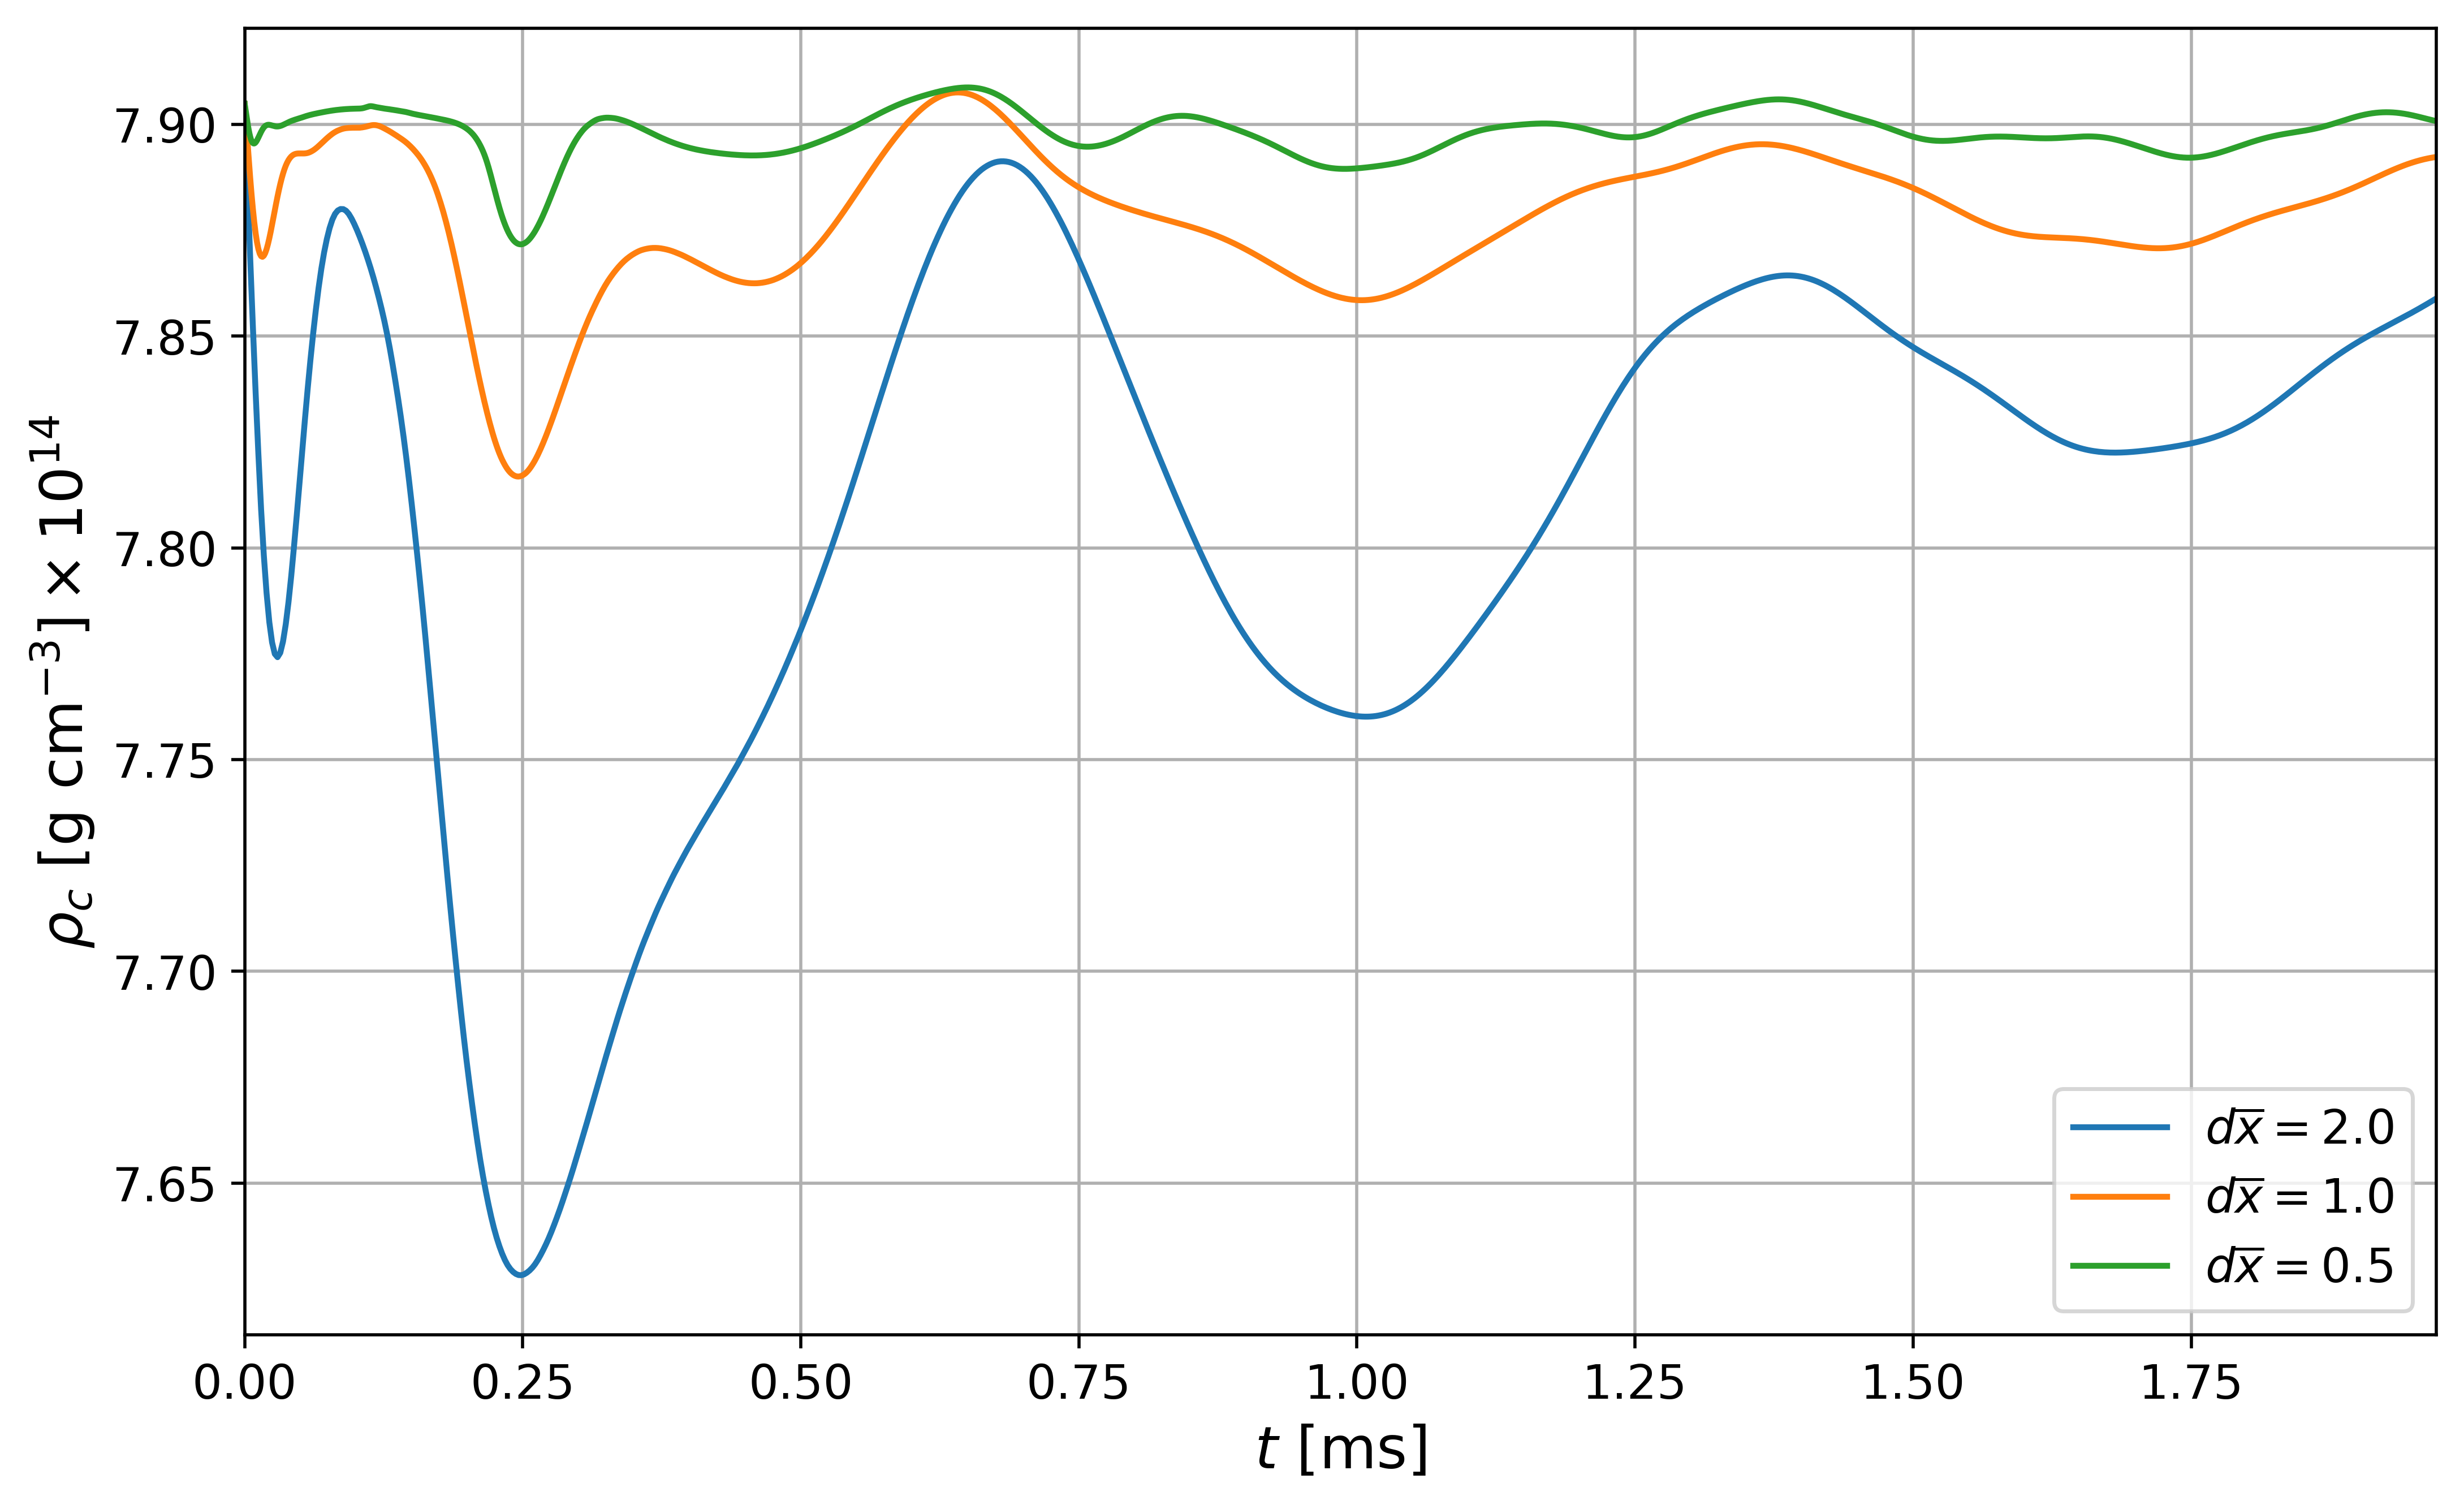
\includegraphics[width=1\linewidth]{images/rhoc_0_rescompare.png}
    \captionof{figure}{Unperturbed \acrshort{ns}; Central density; Time evolution; \figrescompcap.}
    \label{fig:ns_rhoc_0_rescompare}
\end{center}

\begin{center}
    \centering
    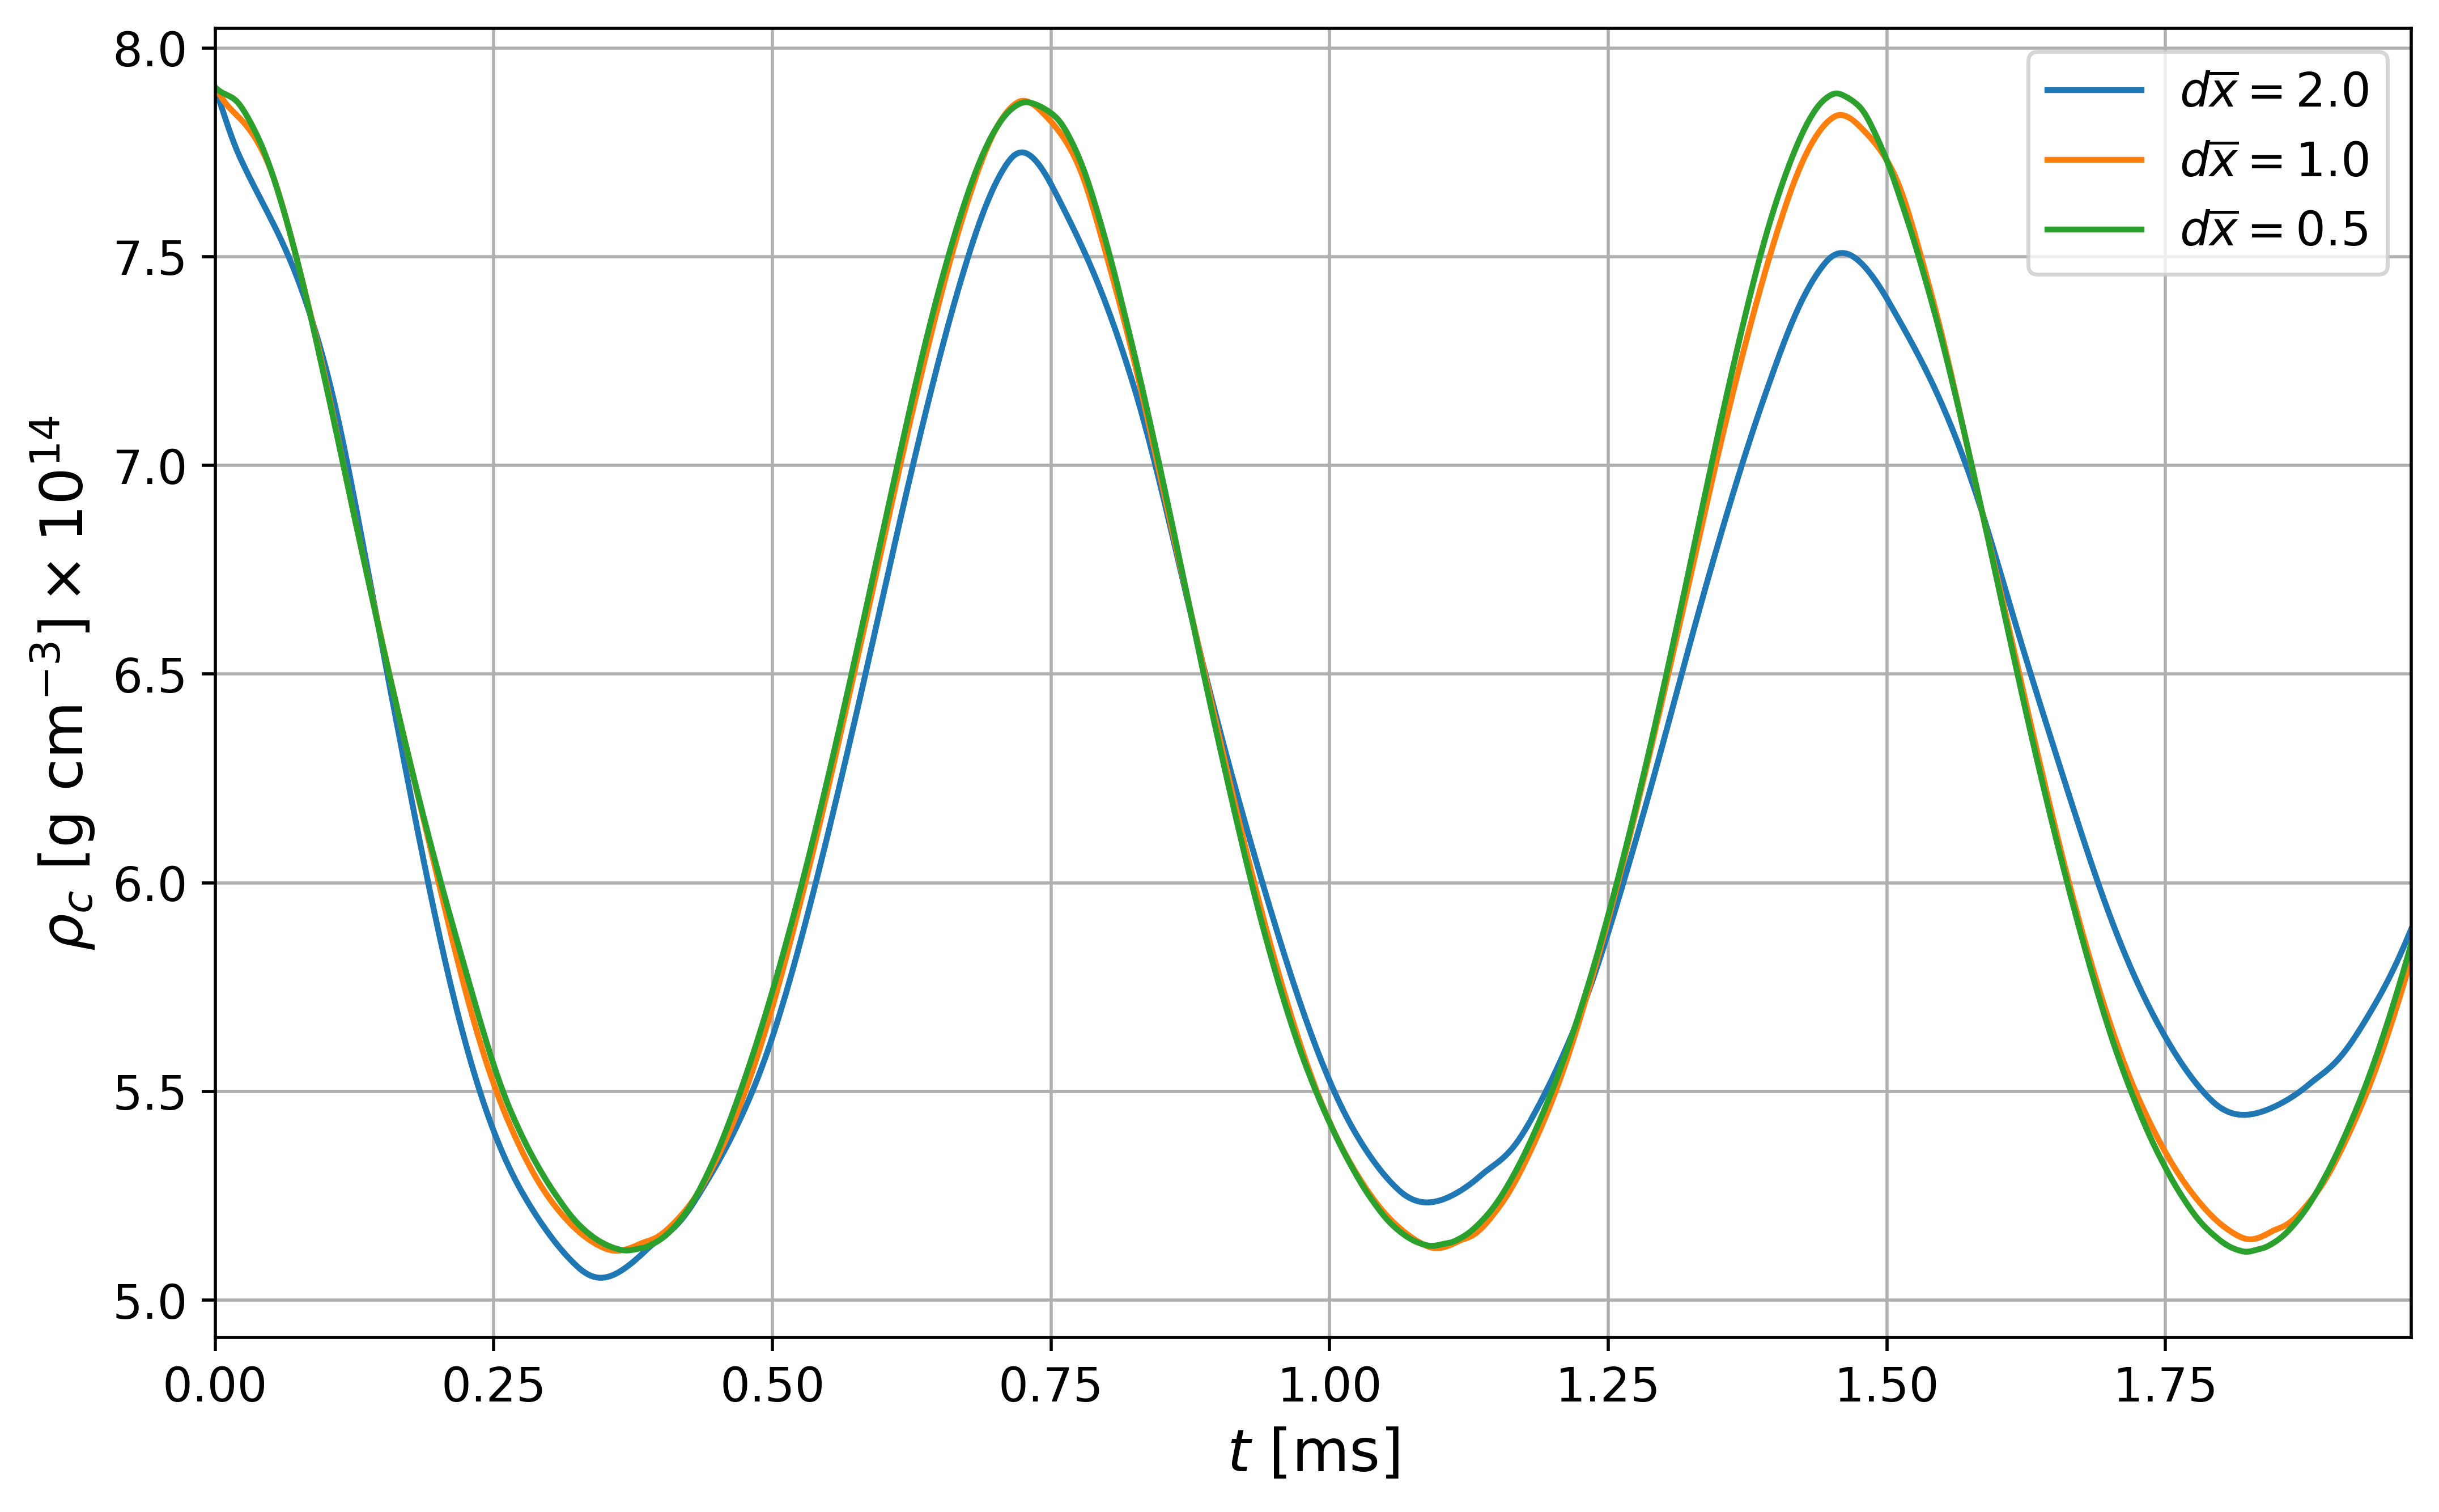
\includegraphics[width=1\linewidth]{images/rhoc_pert_rescompare.png}
    \captionof{figure}{Perturbed \acrshort{ns} (\(K = 110\)); Central density; Time evolution; \figrescompcap.}
    \label{fig:ns_rhoc_pert_110_rescompare}
\end{center}

\begin{center}
    \centering
    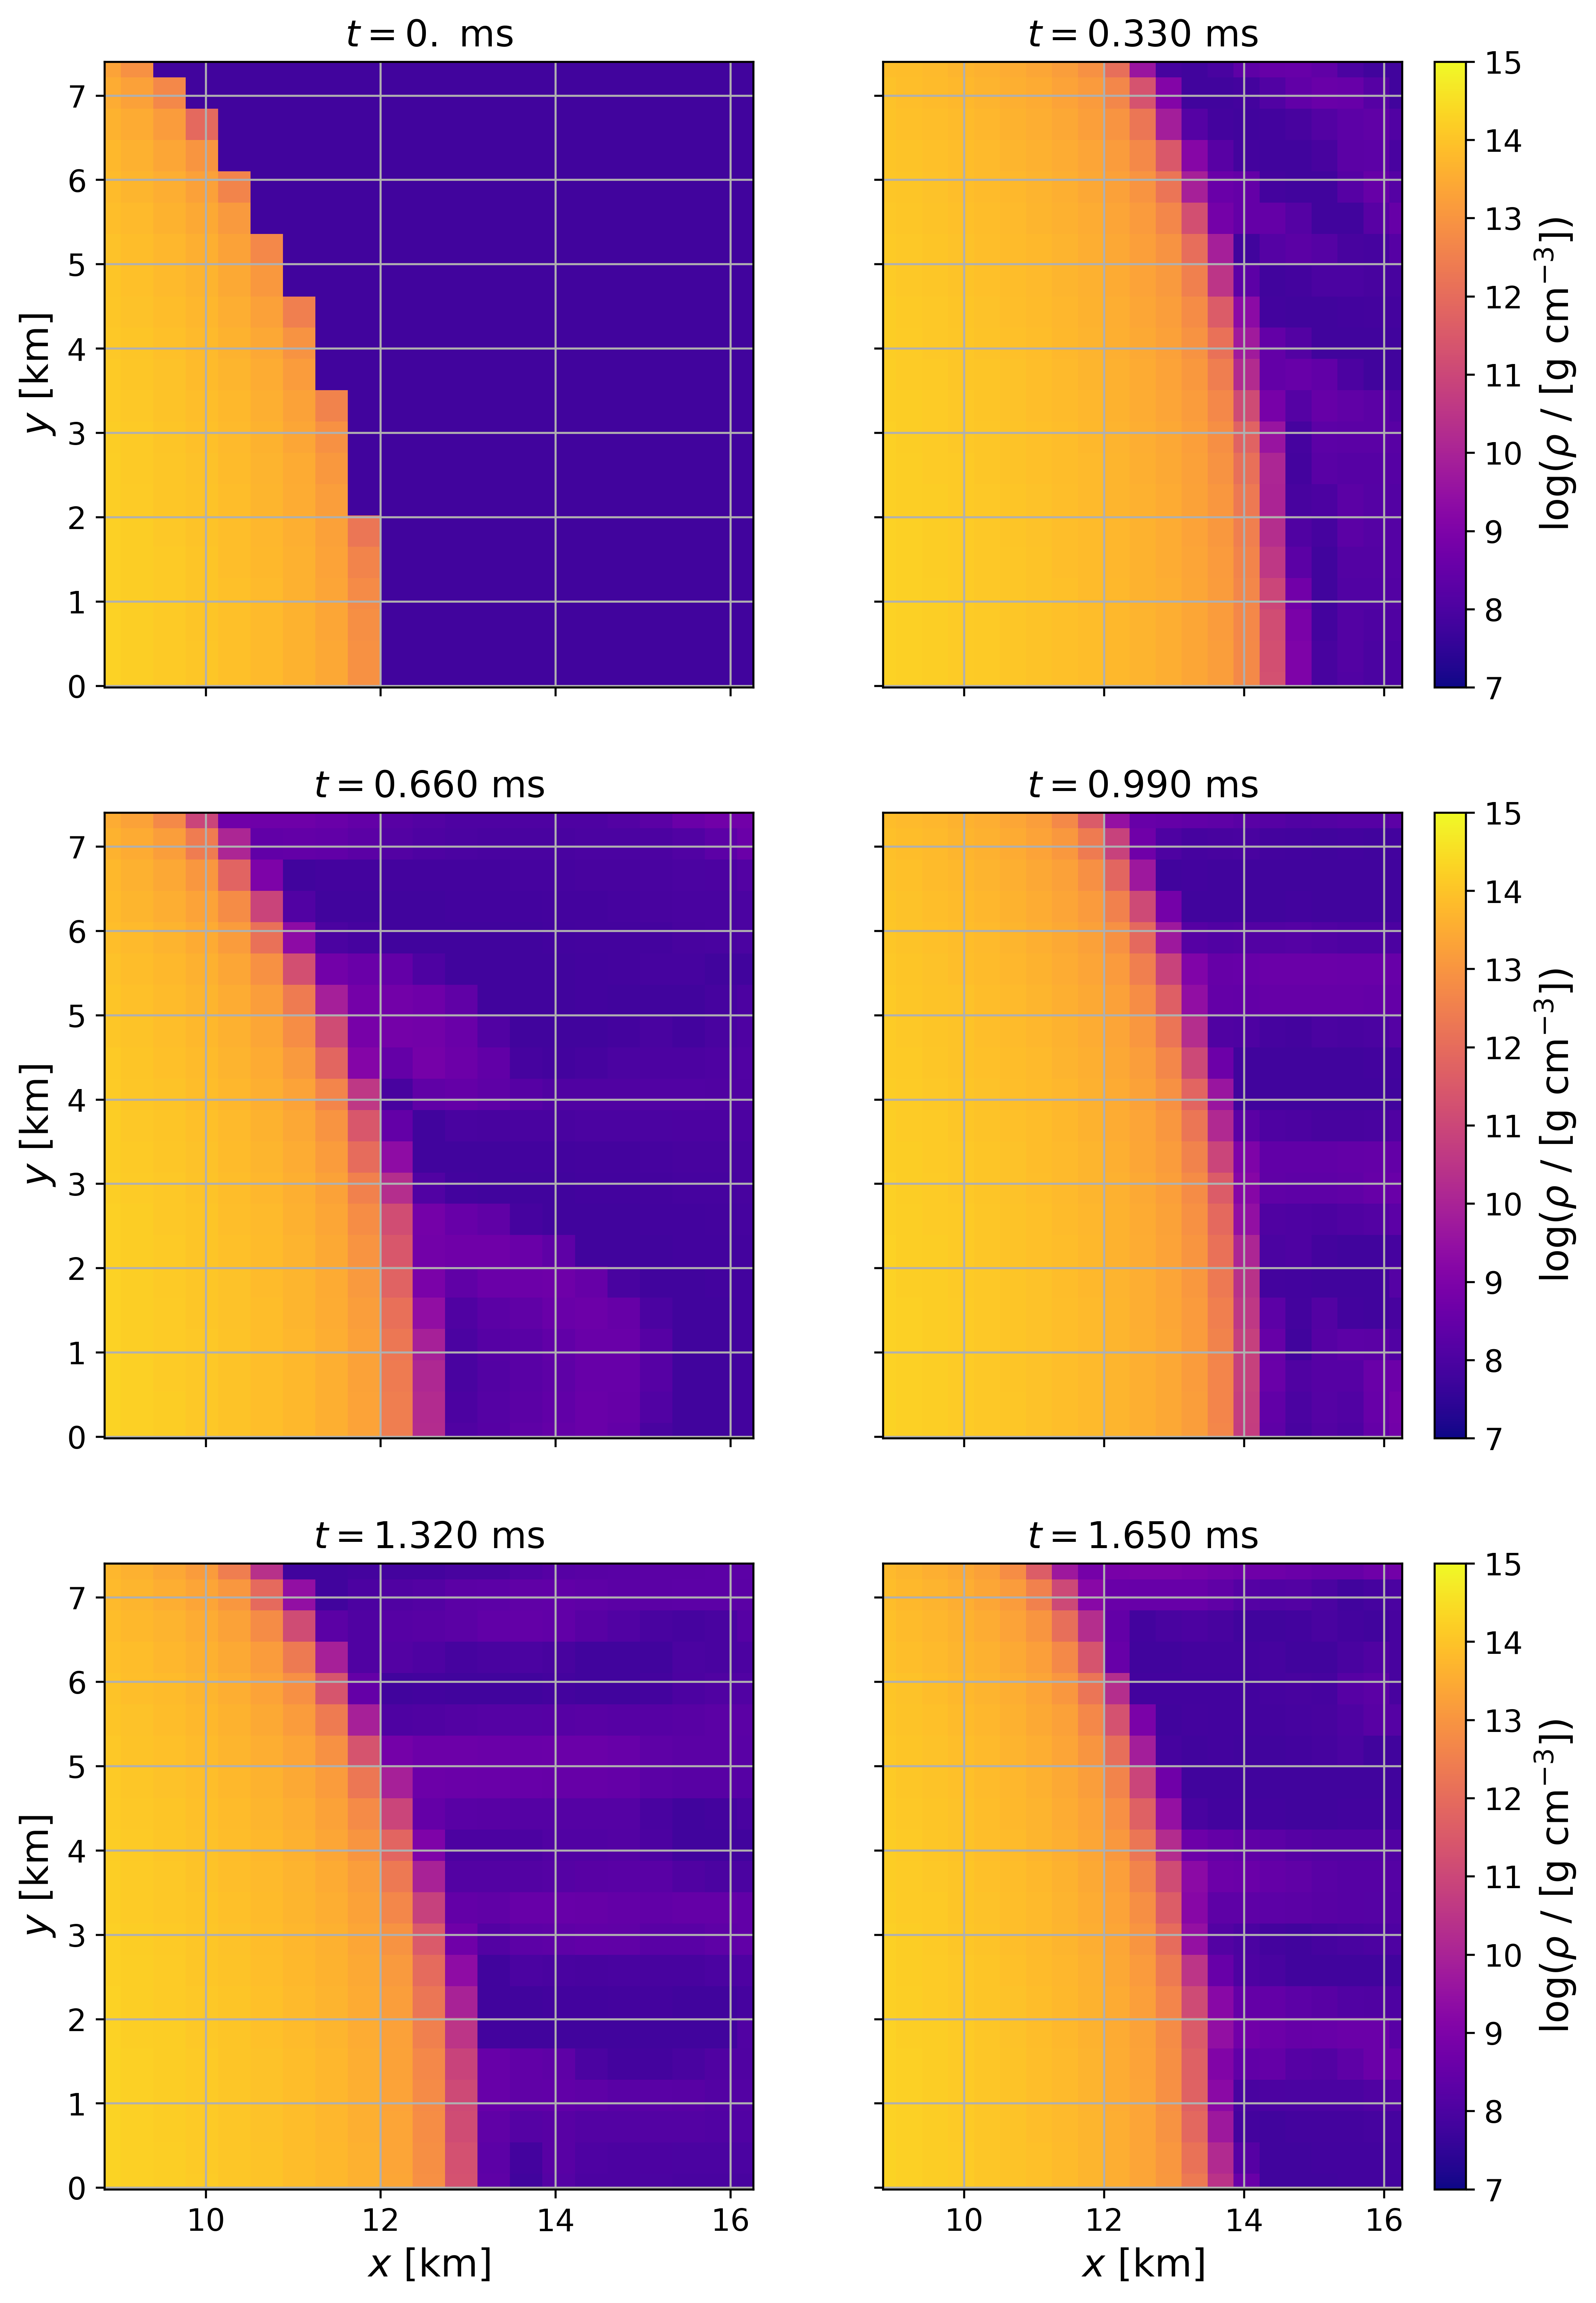
\includegraphics[height=0.9\textheight, width=1\textwidth, keepaspectratio]{images/rho_snapshots.png}
    \captionof{figure}{Perturbed \acrshort{ns} (\(K = 110\)); Rest mass density; Snapshots; Grid spacing = \(0.5\)}
    \label{fig:ns_radial_pulsations}
\end{center}

\begin{center}
    \centering
    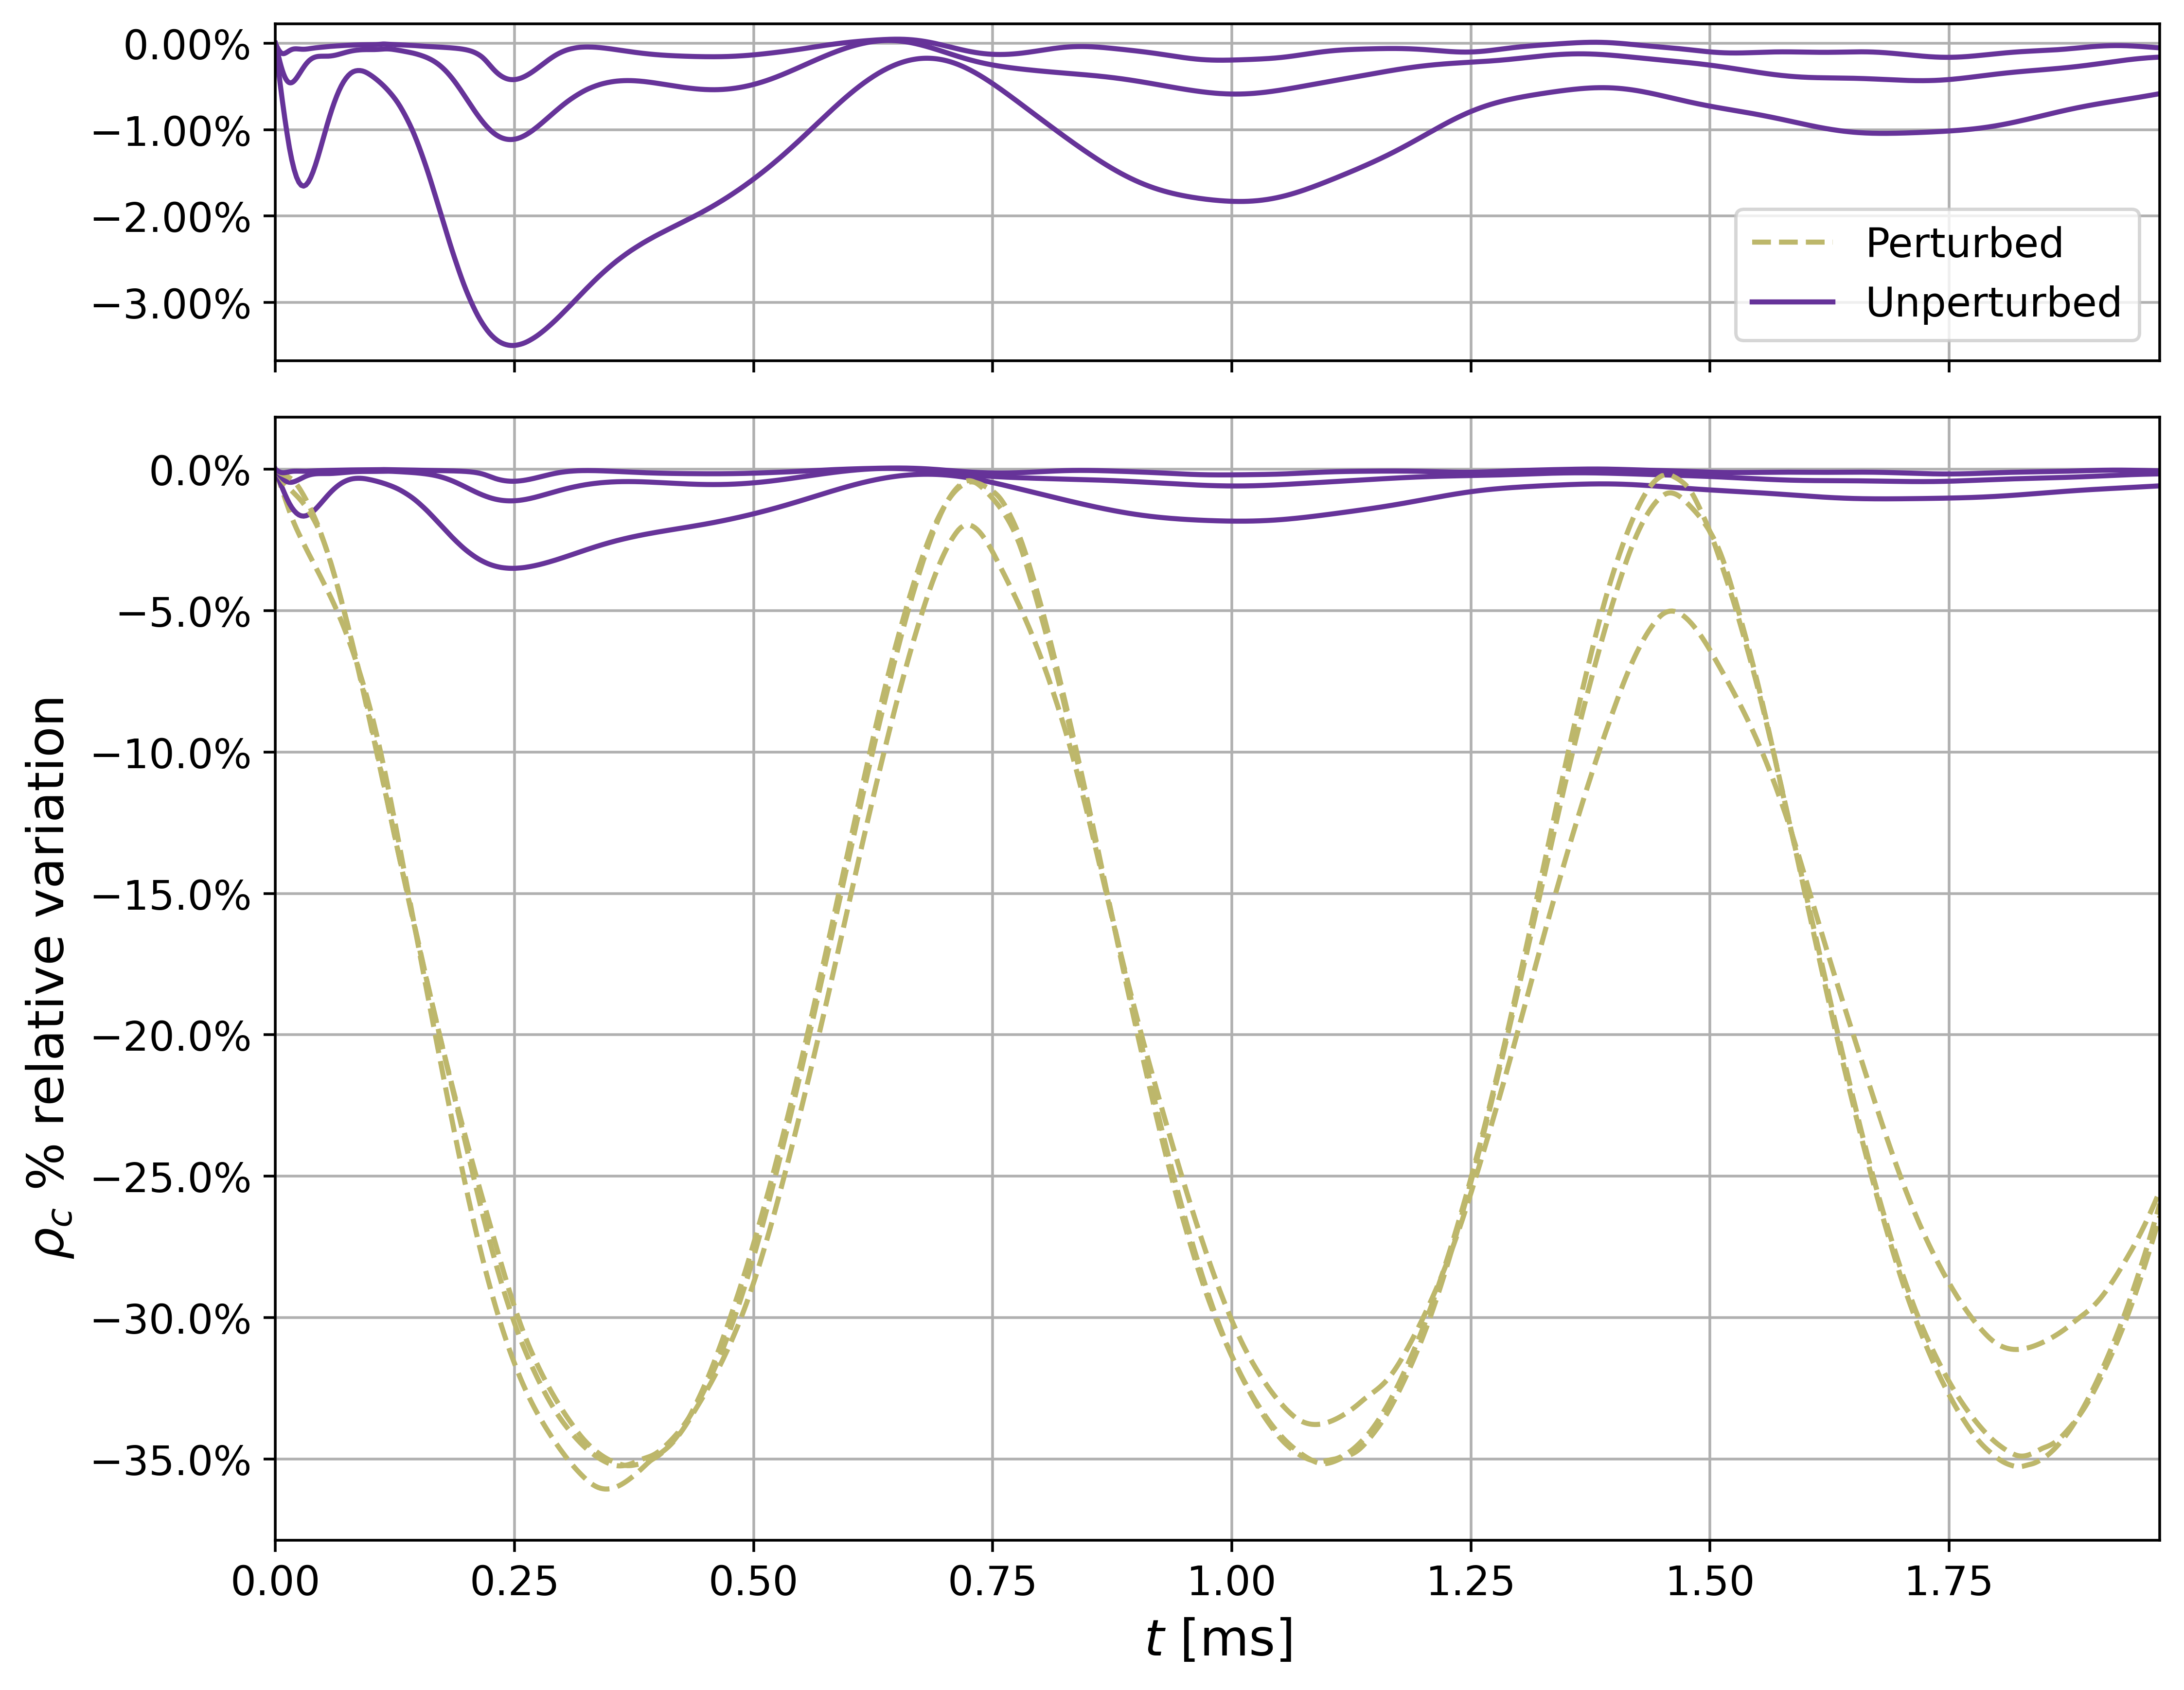
\includegraphics[width=1\linewidth]{images/rhoc_all_typecompare.png}
    \captionof{figure}{Central density; Time evolution; Comparison of perturbed and unperturbed case.}
    \label{fig:ns_rhoc_all_compare}
\end{center}

\newpage

\section{\acrlong{etk} parameters}

\end{document}
